% Part 8: Advanced Topics & Best Practices
% Teaching Agentic Coding Tools to Students
% LaTeX Beamer Presentation with UofSC Color Scheme

\documentclass[aspectratio=169,11pt]{beamer}

% ============================================================
% THEME AND COLOR CONFIGURATION
% ============================================================
\usetheme{Madrid}
\usecolortheme{default}

% Remove rounded corners - sharp edges only
\setbeamertemplate{blocks}[default]
\setbeamertemplate{title page}[default]
\setbeamertemplate{itemize items}[square]
\setbeamertemplate{enumerate items}[default]

% UofSC Color Palette
\definecolor{UofSCGarnet}{HTML}{73000a}
\definecolor{UofSCBlack}{HTML}{000000}
\definecolor{UofSCWhite}{HTML}{ffffff}
\definecolor{UofSCRose}{HTML}{CC2E40}
\definecolor{UofSCAtlantic}{HTML}{466A9F}
\definecolor{UofSCCongaree}{HTML}{1F414D}
\definecolor{UofSCHorseshoe}{HTML}{65780B}
\definecolor{UofSCGrass}{HTML}{CED318}
\definecolor{UofSCHoneycomb}{HTML}{A49137}
\definecolor{UofSC90Black}{HTML}{363636}
\definecolor{UofSC70Black}{HTML}{5C5C5C}
\definecolor{UofSC50Black}{HTML}{A2A2A2}
\definecolor{UofSCWarmGrey}{HTML}{676156}
\definecolor{UofSCSandstorm}{HTML}{FFF2E3}
\definecolor{UofSCDarkGarnet}{HTML}{570008}
\definecolor{UofSCAzalea}{HTML}{844247}

% Apply UofSC colors to Beamer theme
\setbeamercolor{palette primary}{bg=UofSCGarnet,fg=UofSCWhite}
\setbeamercolor{palette secondary}{bg=UofSCCongaree,fg=UofSCWhite}
\setbeamercolor{palette tertiary}{bg=UofSCAtlantic,fg=UofSCWhite}
\setbeamercolor{palette quaternary}{bg=UofSCBlack,fg=UofSCWhite}
\setbeamercolor{structure}{fg=UofSCGarnet}
\setbeamercolor{section in toc}{fg=UofSCBlack}
\setbeamercolor{subsection in toc}{fg=UofSCGarnet}
\setbeamercolor{title}{fg=UofSCWhite,bg=UofSCGarnet}
\setbeamercolor{frametitle}{fg=UofSCWhite,bg=UofSCGarnet}
\setbeamercolor{block title}{bg=UofSCGarnet,fg=UofSCWhite}
\setbeamercolor{block body}{bg=UofSCSandstorm,fg=UofSCBlack}
\setbeamercolor{block title alerted}{bg=UofSCRose,fg=UofSCWhite}
\setbeamercolor{block body alerted}{bg=UofSCSandstorm,fg=UofSCBlack}
\setbeamercolor{block title example}{bg=UofSCAtlantic,fg=UofSCWhite}
\setbeamercolor{block body example}{bg=UofSCSandstorm,fg=UofSCBlack}
\setbeamercolor{itemize item}{fg=UofSCGarnet}
\setbeamercolor{itemize subitem}{fg=UofSCAtlantic}
\setbeamercolor{enumerate item}{fg=UofSCGarnet}
\setbeamercolor{enumerate subitem}{fg=UofSCAtlantic}
\setbeamercolor{normal text}{fg=UofSCBlack,bg=UofSCWhite}
\setbeamercolor{alerted text}{fg=UofSCRose}
\setbeamercolor{example text}{fg=UofSCAtlantic}
\setbeamercolor{footnote}{fg=UofSC70Black}
\setbeamercolor{navigation symbols}{fg=UofSCGarnet}

% ============================================================
% PACKAGES
% ============================================================
\usepackage[utf8]{inputenc}
\usepackage[T1]{fontenc}
\usepackage{lmodern}
\usepackage{tikz}
\usetikzlibrary{shapes.geometric, arrows.meta, positioning, calc, fit, backgrounds, matrix, decorations.pathreplacing}
\usepackage{listings}
\usepackage{xcolor}
\usepackage{graphicx}
\usepackage{hyperref}
\usepackage{booktabs}
\usepackage{array}
\usepackage{multirow}
\usepackage{fontawesome5}

% ============================================================
% LISTINGS CONFIGURATION
% ============================================================
\lstset{
    basicstyle=\ttfamily\scriptsize,
    keywordstyle=\color{UofSCGarnet}\bfseries,
    stringstyle=\color{UofSCAtlantic},
    commentstyle=\color{UofSC70Black}\itshape,
    backgroundcolor=\color{UofSCSandstorm},
    frame=single,
    framerule=0.5pt,
    rulecolor=\color{UofSC50Black},
    breaklines=true,
    breakatwhitespace=true,
    showstringspaces=false,
    tabsize=2,
    xleftmargin=0.5em,
    xrightmargin=0.5em,
    aboveskip=0.5em,
    belowskip=0.5em
}

\lstdefinelanguage{Python}{
    keywords={def, return, if, else, for, in, while, try, except, with, as, import, from, class, True, False, None, and, or, not, is, lambda, yield, assert, break, continue, pass, raise, finally},
    sensitive=true,
    morecomment=[l]{\#},
    morestring=[b]",
    morestring=[b]',
}

\lstdefinelanguage{Bash}{
    keywords={if, then, else, fi, for, in, do, done, while, case, esac, function, return, echo, exit, export, source, cd, ls, git, docker, npm, pip, pytest, python},
    sensitive=true,
    morecomment=[l]{\#},
    morestring=[b]",
    morestring=[b]',
}

\lstdefinelanguage{YAML}{
    keywords={true, false, null},
    sensitive=true,
    morecomment=[l]{\#},
    morestring=[b]",
    morestring=[b]',
}

% ============================================================
% TIKZ STYLES
% ============================================================
\tikzset{
    % Sharp corners for all nodes
    every node/.style={font=\small},
    % Process box style
    process/.style={
        rectangle,
        draw=UofSCBlack,
        fill=UofSCWhite,
        minimum width=2.5cm,
        minimum height=0.8cm,
        align=center,
        font=\footnotesize
    },
    % Decision box style
    decision/.style={
        diamond,
        draw=UofSCBlack,
        fill=UofSCSandstorm,
        minimum width=2cm,
        minimum height=1cm,
        align=center,
        font=\footnotesize,
        aspect=2
    },
    % Start/End style
    startstop/.style={
        rectangle,
        draw=UofSCGarnet,
        fill=UofSCGarnet,
        text=UofSCWhite,
        minimum width=2cm,
        minimum height=0.7cm,
        align=center,
        font=\footnotesize\bfseries
    },
    % Arrow style
    arrow/.style={
        ->,
        >=Stealth,
        thick,
        color=UofSCBlack
    },
    % Failure node
    failure/.style={
        rectangle,
        draw=UofSCRose,
        fill=UofSCRose!20,
        minimum width=2cm,
        minimum height=0.7cm,
        align=center,
        font=\footnotesize
    },
    % Success node
    success/.style={
        rectangle,
        draw=UofSCHorseshoe,
        fill=UofSCHorseshoe!20,
        minimum width=2cm,
        minimum height=0.7cm,
        align=center,
        font=\footnotesize
    },
    % Highlight box
    highlight/.style={
        rectangle,
        draw=UofSCGarnet,
        fill=UofSCGarnet!10,
        line width=1.5pt,
        minimum width=2.5cm,
        minimum height=0.8cm,
        align=center,
        font=\footnotesize
    },
    % Security threat style
    threat/.style={
        rectangle,
        draw=UofSCRose,
        fill=UofSCRose!15,
        minimum width=2.2cm,
        minimum height=0.7cm,
        align=center,
        font=\footnotesize
    },
    % Agent node
    agent/.style={
        rectangle,
        draw=UofSCAtlantic,
        fill=UofSCAtlantic!15,
        minimum width=2.2cm,
        minimum height=0.8cm,
        align=center,
        font=\footnotesize
    },
    % Human node
    human/.style={
        rectangle,
        draw=UofSCCongaree,
        fill=UofSCCongaree!15,
        minimum width=2.2cm,
        minimum height=0.8cm,
        align=center,
        font=\footnotesize
    },
    % Cost node
    cost/.style={
        rectangle,
        draw=UofSCHoneycomb,
        fill=UofSCHoneycomb!20,
        minimum width=2cm,
        minimum height=0.7cm,
        align=center,
        font=\footnotesize
    },
    % Test node
    test/.style={
        rectangle,
        draw=UofSCAtlantic,
        fill=UofSCAtlantic!10,
        minimum width=2cm,
        minimum height=0.7cm,
        align=center,
        font=\footnotesize
    },
    % Pipeline stage
    pipeline/.style={
        rectangle,
        draw=UofSCCongaree,
        fill=UofSCCongaree!10,
        minimum width=2.5cm,
        minimum height=0.8cm,
        align=center,
        font=\footnotesize
    },
    % Timeline event
    timeline/.style={
        rectangle,
        draw=UofSCGarnet,
        fill=UofSCWhite,
        minimum width=1.8cm,
        minimum height=0.6cm,
        align=center,
        font=\tiny
    }
}

% ============================================================
% DOCUMENT INFO
% ============================================================
\title[Part 8: Advanced Topics]{Part 8: Advanced Topics \& Best Practices}
\subtitle{Teaching Agentic Coding Tools to Students}
\author{Graduate Seminar}
\institute{University of South Carolina}
\date{Spring 2026}

% ============================================================
% DOCUMENT
% ============================================================
\begin{document}

% Title Slide
\begin{frame}[plain]
    \titlepage
\end{frame}

% Table of Contents
\begin{frame}{Table of Contents}
    \tableofcontents
\end{frame}

% ============================================================
% SECTION 1: ERROR HANDLING & RECOVERY
% ============================================================
\section{Error Handling \& Recovery}

% Slide 1
\begin{frame}{When Agents Fail: Common Failure Points}
    \begin{columns}[T]
        \begin{column}{0.48\textwidth}
            \textbf{Agents can fail at multiple stages:}
            \begin{itemize}
                \item \textbf{Tool execution failure}: Tool crashes or returns unexpected format
                \item \textbf{Decision-making error}: Agent chooses wrong tool or parameters
                \item \textbf{Token exhaustion}: Context window fills before completion
                \item \textbf{Network/API issues}: External service unavailable
                \item \textbf{Timeout}: Task takes too long
                \item \textbf{Hallucination}: Agent invents non-existent tools
            \end{itemize}
        \end{column}
        \begin{column}{0.48\textwidth}
            \centering
            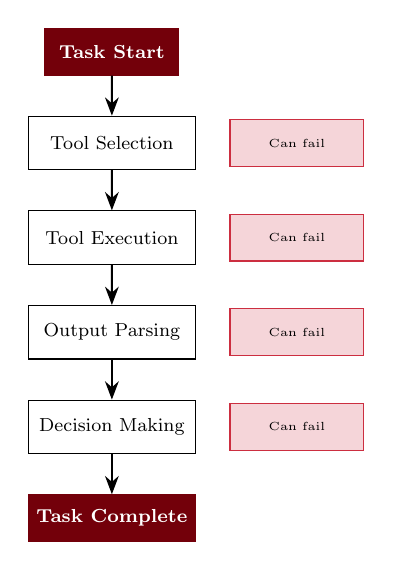
\begin{tikzpicture}[node distance=0.6cm, scale=0.85, transform shape]
                \node (start) [startstop] {Task Start};
                \node (tool) [process, below=of start] {Tool Selection};
                \node (exec) [process, below=of tool] {Tool Execution};
                \node (parse) [process, below=of exec] {Output Parsing};
                \node (decide) [process, below=of parse] {Decision Making};
                \node (end) [startstop, below=of decide] {Task Complete};

                \draw [arrow] (start) -- (tool);
                \draw [arrow] (tool) -- (exec);
                \draw [arrow] (exec) -- (parse);
                \draw [arrow] (parse) -- (decide);
                \draw [arrow] (decide) -- (end);

                % Failure indicators
                \node [failure, right=0.5cm of tool, font=\tiny] {Can fail};
                \node [failure, right=0.5cm of exec, font=\tiny] {Can fail};
                \node [failure, right=0.5cm of parse, font=\tiny] {Can fail};
                \node [failure, right=0.5cm of decide, font=\tiny] {Can fail};
            \end{tikzpicture}
        \end{column}
    \end{columns}

    \note{Start by normalizing failure. Agents will fail - that's not a bug, it's a feature. The best workflows anticipate failures and include recovery strategies.}
\end{frame}

% Slide 2
\begin{frame}[fragile]{Managing Timeouts in Long-Running Tasks}
    \begin{columns}[T]
        \begin{column}{0.52\textwidth}
            \textbf{The Problem:}
            \begin{lstlisting}[language=Bash]
User starts task -> Agent processes
-> 5 minutes pass -> TIMEOUT
Work is lost. Must restart.
            \end{lstlisting}

            \vspace{0.3cm}
            \textbf{Solution 1: Checkpointing}
            \begin{lstlisting}[language=Python]
def run_with_checkpoints(task):
    for chunk in split_task(task):
        result = run_with_timeout(
            chunk, timeout=60)
        save_checkpoint(result)
        if failed(result):
            load_last_checkpoint()
            break
    return combine_results()
            \end{lstlisting}
        \end{column}
        \begin{column}{0.45\textwidth}
            \textbf{Solution 2: Simplification}
            \begin{lstlisting}[language=Bash]
Large task -> Timeout
-> Reduce scope -> Retry
            \end{lstlisting}

            \vspace{0.3cm}
            \begin{block}{Key Insight}
                Break work into natural boundaries:
                \begin{itemize}
                    \item By file
                    \item By function
                    \item By feature
                    \item By batch size
                \end{itemize}
            \end{block}
        \end{column}
    \end{columns}
\end{frame}

% Slide 3
\begin{frame}[fragile]{Recovering from Interruptions and Crashes}
    \begin{columns}[T]
        \begin{column}{0.48\textwidth}
            \textbf{Recovery Pattern - With Git:}
            \begin{lstlisting}[language=Bash]
# During task: commit frequently
git add specific_files.py
git commit -m "checkpoint: X done"

# After interruption:
git log --oneline -10
git status  # See what's incomplete

# Resume with context
            \end{lstlisting}

            \vspace{0.2cm}
            \textbf{Resumption Prompt:}
            \begin{lstlisting}[language=Bash]
We stopped work on this project.
Here's where we left off:
- Completed: [list]
- Remaining: [list]
Continue from where we stopped.
            \end{lstlisting}
        \end{column}
        \begin{column}{0.48\textwidth}
            \textbf{Recovery Pattern - Checkpoint File:}
            \begin{lstlisting}[language=Bash]
{
  "task": "Refactor auth",
  "completed": [
    "Analyzed existing code",
    "Identified functions",
    "Refactored User class"
  ],
  "remaining": [
    "Refactor Token class",
    "Refactor Session class",
    "Write tests"
  ],
  "last_output": "..."
}
            \end{lstlisting}

            \begin{alertblock}{Best Practice}
                Version control is your best recovery mechanism.
            \end{alertblock}
        \end{column}
    \end{columns}
\end{frame}

% Slide 4
\begin{frame}[fragile]{Understanding Why Agents Make Certain Choices}
    \textbf{Debugging Agent Decision-Making}

    \begin{columns}[T]
        \begin{column}{0.32\textwidth}
            \textbf{Strategy 1: Verbose Logging}
            \begin{lstlisting}[language=Bash]
# Request verbose output
"Run with verbose
logging so I can see
your reasoning"

# Look for:
# - Tool selection
# - Parameter choices
# - Rejected approaches
            \end{lstlisting}
        \end{column}
        \begin{column}{0.32\textwidth}
            \textbf{Strategy 2: Thinking Prompts}
            \begin{lstlisting}[language=Bash]
Before you write code,
think through:
1. What is the problem?
2. What are 3 approaches?
3. Which is best? Why?
4. What are pitfalls?
Then implement.
            \end{lstlisting}
        \end{column}
        \begin{column}{0.32\textwidth}
            \textbf{Common Decision Errors:}
            \begin{itemize}
                \item Inefficient tool for task
                \item Incorrect parameters
                \item Wrong file/location
                \item Misunderstood requirement
                \item Over-complicated solution
            \end{itemize}
        \end{column}
    \end{columns}

    \vspace{0.3cm}
    \begin{block}{Debugging Mindset}
        "What would I need to know to make this decision correctly?"
    \end{block}
\end{frame}

% Slide 5
\begin{frame}[fragile]{Managing Context Window Exhaustion}
    \begin{columns}[T]
        \begin{column}{0.55\textwidth}
            \textbf{Token Usage Timeline:}
            \begin{lstlisting}[language=Bash]
Task Start: 2K tokens (prompt + setup)
5 Tool calls: +15K tokens (accumulate)
10 More calls: +30K tokens (growing)
Large file read: +20K tokens
Continue reading: +50K tokens
Agent tries: "Context window exceeded"
            \end{lstlisting}

            \vspace{0.2cm}
            \textbf{Model Limits:}
            \begin{itemize}
                \item Claude 3.5 Haiku: 200K tokens
                \item Claude 3.5 Sonnet: 200K tokens
                \item Claude Opus 4.5: 200K tokens
            \end{itemize}
        \end{column}
        \begin{column}{0.42\textwidth}
            \textbf{Recovery Strategy:}
            \begin{lstlisting}[language=Bash]
# Summarize context
"Summary of completed work:
- Created auth system
- Added 3 middleware
- Fixed 2 bugs

Now we need to: [task]"
            \end{lstlisting}

            \begin{block}{Estimation}
                \begin{itemize}
                    \item Code file: 5-50 tokens/line
                    \item 1000-line file: 5-50K tokens
                    \item Git diff: variable, large
                \end{itemize}
            \end{block}
        \end{column}
    \end{columns}
\end{frame}

% Slide 6
\begin{frame}{Recognizing Repeated Failure Modes}
    \begin{columns}[T]
        \begin{column}{0.48\textwidth}
            \textbf{Pattern 1: The Infinite Loop}
            \begin{itemize}
                \item Agent adds logging to debug
                \item Agent removes feature to fix
                \item Agent reverts changes
                \item Back to original bug...
            \end{itemize}
            \textcolor{UofSCGarnet}{\textbf{Fix:}} Set max iterations. After 3 fails, human intervention.

            \vspace{0.3cm}
            \textbf{Pattern 2: Wrong Tool Syndrome}
            \begin{itemize}
                \item Debug Python with Bash
                \item Modify JS with Python tool
                \item Build with wrong compiler
            \end{itemize}
            \textcolor{UofSCGarnet}{\textbf{Fix:}} Explicitly state which tools are appropriate.
        \end{column}
        \begin{column}{0.48\textwidth}
            \textbf{Pattern 3: Assumption Failure}
            \begin{itemize}
                \item Agent assumes file exists
                \item Doesn't check first
                \item "Error: file not found"
            \end{itemize}
            \textcolor{UofSCGarnet}{\textbf{Fix:}} Always verify preconditions.

            \vspace{0.3cm}
            \textbf{Pattern 4: Scope Creep}
            \begin{itemize}
                \item "I'll fix the bug"
                \item "While here, I'll refactor"
                \item "Actually, let me add features"
                \item Task never completes
            \end{itemize}
            \textcolor{UofSCGarnet}{\textbf{Fix:}} "Fix ONLY the bug. Don't refactor."
        \end{column}
    \end{columns}
\end{frame}

% Slide 7
\begin{frame}{Preventing One Failure from Causing Many}
    \textbf{Handling Cascading Failures}

    \centering
    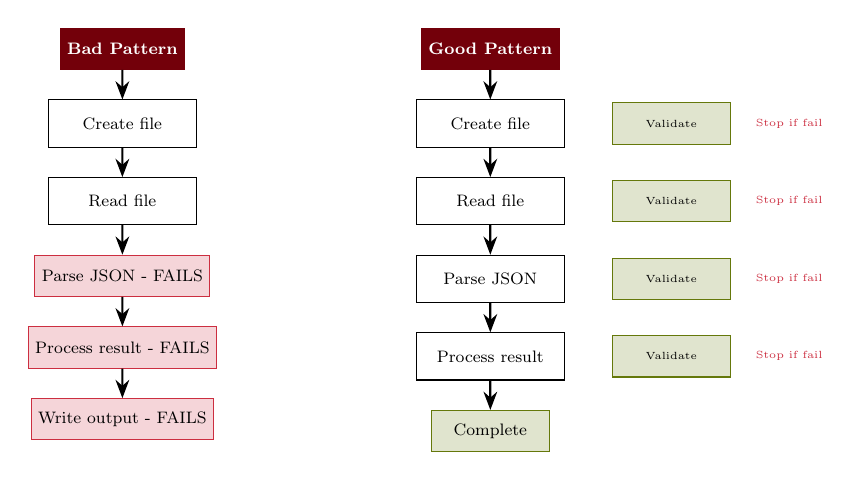
\begin{tikzpicture}[node distance=0.5cm and 1.5cm, scale=0.75, transform shape]
        % Bad pattern
        \node (bad) [startstop] {Bad Pattern};
        \node (b1) [process, below=of bad] {Create file};
        \node (b2) [process, below=of b1] {Read file};
        \node (b3) [failure, below=of b2] {Parse JSON - FAILS};
        \node (b4) [failure, below=of b3] {Process result - FAILS};
        \node (b5) [failure, below=of b4] {Write output - FAILS};

        \draw [arrow] (bad) -- (b1);
        \draw [arrow] (b1) -- (b2);
        \draw [arrow] (b2) -- (b3);
        \draw [arrow] (b3) -- (b4);
        \draw [arrow] (b4) -- (b5);

        % Good pattern
        \node (good) [startstop, right=4cm of bad] {Good Pattern};
        \node (g1) [process, below=of good] {Create file};
        \node (v1) [success, right=0.8cm of g1, font=\tiny] {Validate};
        \node (g2) [process, below=of g1] {Read file};
        \node (v2) [success, right=0.8cm of g2, font=\tiny] {Validate};
        \node (g3) [process, below=of g2] {Parse JSON};
        \node (v3) [success, right=0.8cm of g3, font=\tiny] {Validate};
        \node (g4) [process, below=of g3] {Process result};
        \node (v4) [success, right=0.8cm of g4, font=\tiny] {Validate};
        \node (g5) [success, below=of g4] {Complete};

        \draw [arrow] (good) -- (g1);
        \draw [arrow] (g1) -- (g2);
        \draw [arrow] (g2) -- (g3);
        \draw [arrow] (g3) -- (g4);
        \draw [arrow] (g4) -- (g5);

        % Stop indicators
        \node [font=\tiny\color{UofSCRose}, right=0.3cm of v1] {Stop if fail};
        \node [font=\tiny\color{UofSCRose}, right=0.3cm of v2] {Stop if fail};
        \node [font=\tiny\color{UofSCRose}, right=0.3cm of v3] {Stop if fail};
        \node [font=\tiny\color{UofSCRose}, right=0.3cm of v4] {Stop if fail};
    \end{tikzpicture}

    \vspace{0.3cm}
    \begin{block}{Principle}
        A failure in step 2 should not affect step 4. Validate at each checkpoint.
    \end{block}
\end{frame}

% Slide 8
\begin{frame}[fragile]{Tools and Techniques for Getting Back on Track}
    \textbf{Recovery Strategies}

    \begin{columns}[T]
        \begin{column}{0.48\textwidth}
            \textbf{Strategy 1: Checkpoint \& Restore}
            \begin{lstlisting}[language=Bash]
# Save state
git add . && git commit -m \
  "checkpoint before change"

# If something goes wrong
git reset --hard HEAD~1
git log --oneline -5

# Resume with new approach
            \end{lstlisting}

            \textbf{Strategy 2: Rollback \& Retry}
            \begin{itemize}
                \item Did it work? $\rightarrow$ Move forward
                \item Same error? $\rightarrow$ Different approach
                \item New error? $\rightarrow$ Fix that first
                \item Unclear? $\rightarrow$ Get more info
            \end{itemize}
        \end{column}
        \begin{column}{0.48\textwidth}
            \textbf{Strategy 3: Reduce Scope}
            \begin{lstlisting}[language=Bash]
Original: "Build complete auth"
Failed: "Too many parts"
New: "Build ONLY login endpoint"

Once that works:
"Add user registration"
"Add password reset"
            \end{lstlisting}

            \textbf{Recovery Checklist:}
            \begin{itemize}
                \item[$\square$] Understand what failed and why
                \item[$\square$] Assess if similar to previous
                \item[$\square$] Determine if scope should reduce
                \item[$\square$] Provide additional context
                \item[$\square$] Set iteration limit
            \end{itemize}
        \end{column}
    \end{columns}
\end{frame}

% Slide 9
\begin{frame}{What NOT to Do When Agents Fail}
    \textbf{Anti-Patterns to Avoid}

    \begin{columns}[T]
        \begin{column}{0.48\textwidth}
            \begin{alertblock}{Anti-Pattern 1: Ignoring the Error}
                \textbf{Bad:} "Just continue anyway"\\
                \textbf{Better:} "The file wasn't found. Let me tell you where it is."
            \end{alertblock}

            \begin{alertblock}{Anti-Pattern 2: Over-Specifying Recovery}
                \textbf{Bad:} "Do X. If fails do Y. If fails do Z..."\\
                \textbf{Better:} "Try X. If fails, stop and tell me."
            \end{alertblock}

            \begin{alertblock}{Anti-Pattern 3: Silent Failures}
                \textbf{Bad:} Agent silently continues\\
                \textbf{Good:} Agent reports what succeeded/failed
            \end{alertblock}
        \end{column}
        \begin{column}{0.48\textwidth}
            \begin{alertblock}{Anti-Pattern 4: Changing Strategy Mid-Stream}
                \textbf{Bad:} "Refactor" $\rightarrow$ "Rewrite" $\rightarrow$ "Just fix bug"\\
                \textbf{Better:} Plan the strategy upfront.
            \end{alertblock}

            \begin{alertblock}{Anti-Pattern 5: Assuming Agent Knowledge}
                \textbf{Bad:} "Fix following RESTful principles"\\
                \textbf{Better:} "Fix following RESTful principles. Here's an example: [code]"
            \end{alertblock}

            \vspace{0.3cm}
            \begin{block}{Key Insight}
                Anti-patterns are born from impatience. Stop and ask: "Is there a better way?"
            \end{block}
        \end{column}
    \end{columns}
\end{frame}

% Slide 10
\begin{frame}{Designing for Failure from the Start}
    \textbf{Building Fault-Tolerant Workflows}

    \centering
    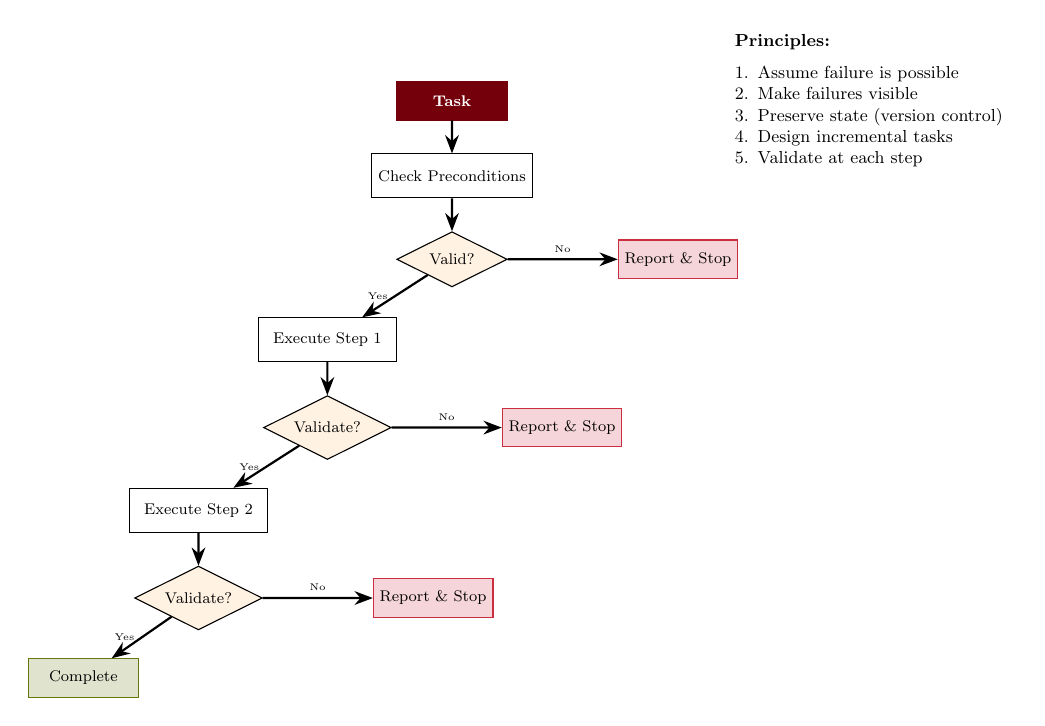
\begin{tikzpicture}[node distance=0.6cm and 2cm, scale=0.7, transform shape]
        % Error Recovery Workflow
        \node (task) [startstop] {Task};
        \node (pre) [process, below=of task] {Check Preconditions};
        \node (d1) [decision, below=of pre] {Valid?};
        \node (step1) [process, below left=0.8cm and 0.5cm of d1] {Execute Step 1};
        \node (fail1) [failure, right=2cm of d1] {Report \& Stop};
        \node (v1) [decision, below=of step1] {Validate?};
        \node (step2) [process, below left=0.8cm and 0.5cm of v1] {Execute Step 2};
        \node (fail2) [failure, right=2cm of v1] {Report \& Stop};
        \node (v2) [decision, below=of step2] {Validate?};
        \node (complete) [success, below left=0.8cm and 0.5cm of v2] {Complete};
        \node (fail3) [failure, right=2cm of v2] {Report \& Stop};

        \draw [arrow] (task) -- (pre);
        \draw [arrow] (pre) -- (d1);
        \draw [arrow] (d1) -- node[left, font=\tiny] {Yes} (step1);
        \draw [arrow] (d1) -- node[above, font=\tiny] {No} (fail1);
        \draw [arrow] (step1) -- (v1);
        \draw [arrow] (v1) -- node[left, font=\tiny] {Yes} (step2);
        \draw [arrow] (v1) -- node[above, font=\tiny] {No} (fail2);
        \draw [arrow] (step2) -- (v2);
        \draw [arrow] (v2) -- node[left, font=\tiny] {Yes} (complete);
        \draw [arrow] (v2) -- node[above, font=\tiny] {No} (fail3);

        % Principles on the right
        \node [right=4cm of task, text width=5cm, font=\small] {
            \textbf{Principles:}\\[0.2cm]
            1. Assume failure is possible\\
            2. Make failures visible\\
            3. Preserve state (version control)\\
            4. Design incremental tasks\\
            5. Validate at each step
        };
    \end{tikzpicture}
\end{frame}

% ============================================================
% SECTION 2: SECURITY & SAFETY
% ============================================================
\section{Security \& Safety}

% Slide 11
\begin{frame}{Agents Have Full System Access: What Could Go Wrong?}
    \textbf{Understanding Agent Security Risks}

    \begin{columns}[T]
        \begin{column}{0.45\textwidth}
            \textbf{Critical Reality:}
            When you give an agent access:
            \begin{itemize}
                \item Read all your files (including keys, secrets)
                \item Modify any file
                \item Execute any command
                \item Delete files
                \item Network requests (download/upload)
                \item Install software
                \item Create backdoors
                \item Exfiltrate data
            \end{itemize}

            \begin{alertblock}{Trust Model}
                The agent operates with YOUR permissions.
            \end{alertblock}
        \end{column}
        \begin{column}{0.52\textwidth}
            \centering
            \textbf{Security Threat Model}

            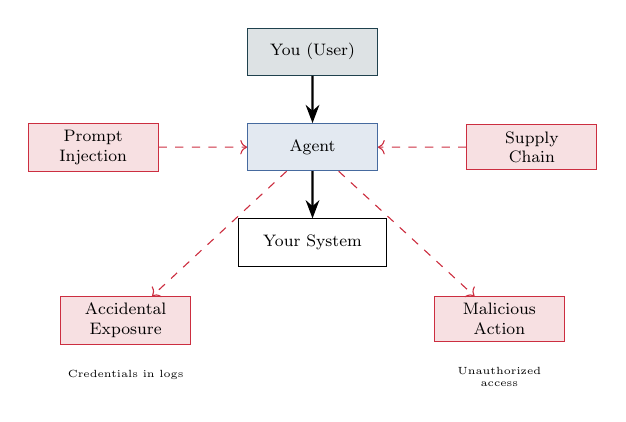
\begin{tikzpicture}[node distance=0.8cm, scale=0.75, transform shape]
                \node (you) [human] {You (User)};
                \node (agent) [agent, below=of you] {Agent};
                \node (system) [process, below=of agent] {Your System};

                \draw [arrow] (you) -- (agent);
                \draw [arrow] (agent) -- (system);

                % Threat vectors
                \node (t1) [threat, left=1.5cm of agent] {Prompt\\Injection};
                \node (t2) [threat, right=1.5cm of agent] {Supply\\Chain};
                \node (t3) [threat, below left=0.5cm and 0.8cm of system] {Accidental\\Exposure};
                \node (t4) [threat, below right=0.5cm and 0.8cm of system] {Malicious\\Action};

                \draw [->, dashed, color=UofSCRose] (t1) -- (agent);
                \draw [->, dashed, color=UofSCRose] (t2) -- (agent);
                \draw [->, dashed, color=UofSCRose] (agent) -- (t3);
                \draw [->, dashed, color=UofSCRose] (agent) -- (t4);

                \node [below=0.3cm of t3, font=\tiny, text width=2cm, align=center] {Credentials in logs};
                \node [below=0.3cm of t4, font=\tiny, text width=2cm, align=center] {Unauthorized access};
            \end{tikzpicture}
        \end{column}
    \end{columns}
\end{frame}

% Slide 12
\begin{frame}[fragile]{Strategies to Prevent Harmful Agent Actions}
    \textbf{Preventing Malicious Code Execution}

    \begin{columns}[T]
        \begin{column}{0.48\textwidth}
            \textbf{Strategy 1: Explicit Authorization}
            \begin{lstlisting}[language=Bash]
"Before executing commands
that modify files, ask me
for approval and show the
exact command you plan to run."
            \end{lstlisting}

            \textbf{Strategy 2: Restricted Scope}
            \begin{lstlisting}[language=Bash]
# Better:
"You can run: git, python, npm
 You CANNOT: sudo, rm, install
 packages without asking"
            \end{lstlisting}
        \end{column}
        \begin{column}{0.48\textwidth}
            \textbf{Strategy 3: Command Whitelisting}

            \begin{tabular}{ll}
                \textcolor{UofSCHorseshoe}{\checkmark} & ls, cd, pwd (navigation)\\
                \textcolor{UofSCHorseshoe}{\checkmark} & cat, grep (reading)\\
                \textcolor{UofSCHorseshoe}{\checkmark} & python, node (interpreters)\\
                \textcolor{UofSCHorseshoe}{\checkmark} & git (version control)\\
                \textcolor{UofSCHorseshoe}{\checkmark} & pytest, npm test (testing)\\
                \hline
                \textcolor{UofSCRose}{\texttimes} & sudo (privilege escalation)\\
                \textcolor{UofSCRose}{\texttimes} & rm -rf (destructive)\\
                \textcolor{UofSCRose}{\texttimes} & curl (might exfiltrate)\\
                \textcolor{UofSCRose}{\texttimes} & pip install (malicious pkg)\\
            \end{tabular}

            \vspace{0.3cm}
            \begin{block}{Principle}
                Make attacks expensive and obvious.
            \end{block}
        \end{column}
    \end{columns}
\end{frame}

% Slide 13
\begin{frame}[fragile]{Protecting Secrets While Using Agents}
    \textbf{Handling Sensitive Data}

    \begin{columns}[T]
        \begin{column}{0.48\textwidth}
            \textbf{Strategy 1: Environment Separation}
            \begin{lstlisting}[language=Bash]
# Before invoking agent:
unset AWS_ACCESS_KEY_ID
unset AWS_SECRET_ACCESS_KEY
unset DATABASE_PASSWORD

# Invoke with limited env:
env -i HOME=$HOME USER=$USER \
    SHELL=$SHELL agent-command
            \end{lstlisting}

            \textbf{Strategy 2: Use .claudeignore}
            \begin{lstlisting}[language=Bash]
# .claudeignore
.env
.env.local
.aws/
.ssh/
private_keys/
secrets/
            \end{lstlisting}
        \end{column}
        \begin{column}{0.48\textwidth}
            \textbf{Strategy 3: Redact Sensitive Info}
            \begin{lstlisting}[language=Bash]
# BAD:
DATABASE_URL=postgresql://
  admin:password123@
  db.prod.company.com/prod

# GOOD:
DATABASE_URL=postgresql://
  admin:REDACTED@
  example.com/example_db
            \end{lstlisting}

            \textbf{Strategy 4: Temporary Credentials}
            \begin{lstlisting}[language=Bash]
# Generate temporary creds:
aws sts get-session-token \
  --duration-seconds 900
# Expires after 15 minutes
            \end{lstlisting}
        \end{column}
    \end{columns}
\end{frame}

% Slide 14
\begin{frame}[fragile]{Writing Prompts That Can't Be Exploited}
    \textbf{Safe Prompting Practices}

    \begin{columns}[T]
        \begin{column}{0.48\textwidth}
            \textbf{Principle 1: Explicit is Better}
            \begin{lstlisting}[language=Bash]
# Weak:
"Add validation to this endpoint"

# Strong:
"Add validation to POST /users:
- Validate email format
- Password >= 8 characters
- Name is not empty
Do NOT change endpoint URL.
Do NOT change response format.
Do NOT add new endpoints."
            \end{lstlisting}
        \end{column}
        \begin{column}{0.48\textwidth}
            \textbf{Dangerous Prompts to Avoid:}
            \begin{itemize}
                \item[\textcolor{UofSCRose}{\texttimes}] "Do whatever you think is best"
                \item[\textcolor{UofSCRose}{\texttimes}] "Make this awesome"
                \item[\textcolor{UofSCRose}{\texttimes}] "Optimize everything"
                \item[\textcolor{UofSCRose}{\texttimes}] "Fix all the issues"
                \item[\textcolor{UofSCRose}{\texttimes}] "Make it production-ready"
                \item[\textcolor{UofSCRose}{\texttimes}] "I trust you to handle this"
            \end{itemize}

            \begin{exampleblock}{Better:}
                "Reduce query time by:\\
                1. Adding indexes to user\_id\\
                2. Caching frequent queries\\
                Test with: pytest tests/performance/"
            \end{exampleblock}
        \end{column}
    \end{columns}
\end{frame}

% Slide 15
\begin{frame}{Pre-Flight Security Review}
    \textbf{Security Checklist for Agentic Workflows}

    \begin{columns}[T]
        \begin{column}{0.32\textwidth}
            \textbf{Code \& Data Security:}
            \begin{itemize}
                \item[$\square$] Review prompt for unusual instructions
                \item[$\square$] Confirm no hidden instructions
                \item[$\square$] Verify no sensitive data exposed
                \item[$\square$] Check .gitignore/.claudeignore
                \item[$\square$] Ensure credentials not in env
            \end{itemize}
        \end{column}
        \begin{column}{0.32\textwidth}
            \textbf{System Access Control:}
            \begin{itemize}
                \item[$\square$] Agent has only needed access
                \item[$\square$] Cannot execute arbitrary commands
                \item[$\square$] Cannot install packages
                \item[$\square$] Cannot access \~{}/.ssh or \~{}/.aws
                \item[$\square$] Network restricted
            \end{itemize}
        \end{column}
        \begin{column}{0.32\textwidth}
            \textbf{Monitoring \& Recovery:}
            \begin{itemize}
                \item[$\square$] Can see agent commands
                \item[$\square$] Can see file modifications
                \item[$\square$] Can interrupt immediately
                \item[$\square$] Have rollback plan
                \item[$\square$] Recent git commit exists
            \end{itemize}
        \end{column}
    \end{columns}

    \vspace{0.4cm}
    \begin{exampleblock}{Example: Pre-Flight Check}
        Task: "Refactor authentication module"\\
        \checkmark{} Credentials in .claudeignore \checkmark{} AWS keys unset \checkmark{} Agent restricted to /src/auth/ \checkmark{} Last commit saved $\rightarrow$ \textbf{SAFE TO PROCEED}
    \end{exampleblock}
\end{frame}

% Slide 16
\begin{frame}[fragile]{Responding to Security Incidents with Agents}
    \textbf{Incident Response}

    \begin{columns}[T]
        \begin{column}{0.48\textwidth}
            \textbf{Scenario: Agent Exposed Credentials}

            \textbf{Immediate (5 min):}
            \begin{enumerate}
                \item Kill the agent process
                \item Note what was exposed
                \item Screenshot the response
            \end{enumerate}

            \textbf{Short-term (30 min):}
            \begin{enumerate}
                \item Rotate all exposed credentials
                \item Check CloudTrail for unauthorized access
                \item Check git history for committed keys
            \end{enumerate}

            \textbf{Long-term (24 hr):}
            \begin{enumerate}
                \item Audit similar configurations
                \item Set up secret scanning in CI/CD
                \item Post-mortem: How to prevent?
            \end{enumerate}
        \end{column}
        \begin{column}{0.48\textwidth}
            \textbf{Incident Report Template:}
            \begin{lstlisting}[language=Bash]
Date: 2026-01-23
Time: 14:30 UTC

What happened:
[Description]

How it was discovered:
[Alert source]

Immediate actions taken:
- [Action 1]
- [Action 2]

Credentials affected:
- [List]

Root cause:
[Why it happened]

Prevention:
[Future measures]

Status: RESOLVED
            \end{lstlisting}
        \end{column}
    \end{columns}
\end{frame}

% Slide 17
\begin{frame}[fragile]{Your Agent Security Rules}
    \textbf{Building a Personal Security Policy}

    \begin{columns}[T]
        \begin{column}{0.48\textwidth}
            \begin{lstlisting}[language=Bash]
MY AGENT USAGE POLICY
Updated: [Date]

1. ALLOWED AGENTS
   - Claude Code (terminal)
   - Aider (code editor)

2. ALLOWED TOOLS
   [x] File read/write
   [x] Terminal: git, python, npm
   [ ] Network requests: limited
   [ ] Package install: NO

3. FORBIDDEN ACTIONS
   - Execute in /etc or /root
   - Access ~/.ssh or ~/.aws
   - Network outside approved list
   - Install packages
   - Modify outside /project/
            \end{lstlisting}
        \end{column}
        \begin{column}{0.48\textwidth}
            \begin{lstlisting}[language=Bash]
4. CREDENTIALS HANDLING
   - Keep .env in .claudeignore
   - Rotate before agent work
   - Use temporary credentials
   - Never include in prompts

5. MONITORING REQUIRED
   - Before: Review agent access
   - During: Watch for unusual
   - After: Audit git diff

6. INCIDENT RESPONSE
   If something goes wrong:
   [Steps to follow]
   Report to: [Contact]

7. REVIEW SCHEDULE
   Review: Monthly

Signed: [Your name]
            \end{lstlisting}
        \end{column}
    \end{columns}
\end{frame}

% Slide 18
\begin{frame}{Keeping Agent Usage Secure Over Time}
    \textbf{Long-Term Security Maintenance}

    \begin{columns}[T]
        \begin{column}{0.48\textwidth}
            \textbf{Monthly:}
            \begin{itemize}
                \item Review credentials in system
                \item Audit \~{}/.aws, \~{}/.ssh, .env files
                \item Verify .gitignore and .claudeignore
                \item Check git log for committed secrets
            \end{itemize}

            \vspace{0.3cm}
            \textbf{Quarterly:}
            \begin{itemize}
                \item Review incidents from past 3 months
                \item Update personal security policy
                \item Learn from problems
                \item Share lessons with team
            \end{itemize}
        \end{column}
        \begin{column}{0.48\textwidth}
            \textbf{When Onboarding New Tools:}
            \begin{enumerate}
                \item Evaluate: What access does it need?
                \item Restrict: Give minimum necessary
                \item Monitor: Set up logging/alerting
                \item Document: Add to policy
            \end{enumerate}

            \vspace{0.3cm}
            \textbf{Security Culture:}
            \begin{itemize}
                \item[\textcolor{UofSCRose}{\texttimes}] "Security is IT's job"
                \item[\textcolor{UofSCHorseshoe}{\checkmark}] "Security is everyone's responsibility"
            \end{itemize}

            \begin{block}{Indicators of Good Culture}
                People ask "is this secure?" before proceeding. Incidents are discussed openly.
            \end{block}
        \end{column}
    \end{columns}
\end{frame}

% ============================================================
% SECTION 3: COST MANAGEMENT & OPTIMIZATION
% ============================================================
\section{Cost Management \& Optimization}

% Slide 19
\begin{frame}{Economics of Agentic Workflows}
    \textbf{Understanding Agent Costs}

    \begin{columns}[T]
        \begin{column}{0.48\textwidth}
            \textbf{Cost Structure (per 1M tokens):}

            \begin{tabular}{lccc}
                \toprule
                & Input & Output\\
                \midrule
                Haiku & \$0.80 & \$4.00\\
                Sonnet & \$3.00 & \$15.00\\
                Opus & \$15.00 & \$60.00\\
                \bottomrule
            \end{tabular}

            \vspace{0.3cm}
            \textbf{Real-world Example:}
            \begin{itemize}
                \item Prompt: 5,000 tokens
                \item Tool calls: 20,000 tokens
                \item Response: 8,000 tokens
                \item Total: 33,000 tokens
                \item Cost (Haiku): \textasciitilde\$0.12
            \end{itemize}
        \end{column}
        \begin{column}{0.48\textwidth}
            \textbf{Where Costs Hide:}
            \begin{enumerate}
                \item \textbf{Context Accumulation}\\
                First exchange: 5K $\rightarrow$ 10th exchange: 50K+

                \item \textbf{Tool Outputs}\\
                Read large file: +10K tokens\\
                Run complex command: +5K per output

                \item \textbf{Debugging Iterations}\\
                3 attempts = 3x base cost

                \item \textbf{Retries \& Restarts}\\
                Bad prompt: 20K wasted\\
                New session: Another 20K
            \end{enumerate}

            \begin{alertblock}{Key Insight}
                50\% savings possible with clear prompts.
            \end{alertblock}
        \end{column}
    \end{columns}
\end{frame}

% Slide 20
\begin{frame}[fragile]{Measuring What You're Actually Spending}
    \textbf{Token Usage Tracking and Monitoring}

    \begin{columns}[T]
        \begin{column}{0.48\textwidth}
            \textbf{Claude API (Programmatic):}
            \begin{lstlisting}[language=Python]
from anthropic import Anthropic

client = Anthropic()
response = client.messages.create(
    model="claude-3-5-sonnet",
    max_tokens=1024,
    messages=[{"role": "user",
               "content": "Hello"}]
)

print(f"Input: {response.usage
        .input_tokens}")
print(f"Output: {response.usage
        .output_tokens}")
            \end{lstlisting}
        \end{column}
        \begin{column}{0.48\textwidth}
            \textbf{Monthly Tracking:}

            \begin{tabular}{lr}
                \toprule
                Week & Cost\\
                \midrule
                Week 1 & \$15.42\\
                Week 2 & \$12.80\\
                Week 3 & \$18.92 (spike)\\
                Week 4 & \$8.44\\
                \midrule
                \textbf{Total} & \textbf{\$55.58}\\
                \bottomrule
            \end{tabular}

            \vspace{0.3cm}
            \textbf{Alert Thresholds:}
            \begin{itemize}
                \item Daily: >\$5 (unusual)
                \item Weekly: >\$30 (intensive)
                \item Monthly: >\$150 (project-focused)
            \end{itemize}
        \end{column}
    \end{columns}
\end{frame}

% Slide 21
\begin{frame}[fragile]{Writing Cheaper Prompts}
    \textbf{Optimizing Prompts for Efficiency}

    \begin{columns}[T]
        \begin{column}{0.48\textwidth}
            \textbf{BAD PROMPT (Many iterations):}
            \begin{lstlisting}[language=Bash]
User: "Help me fix this code"
Agent: "What code? What's wrong?"
User: "Python authentication"
Agent: "What specifically?"
User: "Password hashing not working"
Agent: "Here's how to debug..."
Total: ~50K tokens for confusion
            \end{lstlisting}

            \textbf{GOOD PROMPT (One iteration):}
            \begin{lstlisting}[language=Bash]
"Fix password hashing in Python
auth module.
Currently: Using MD5 (insecure)
Should be: Using bcrypt
Files: auth/hash.py, auth/verify.py
Tests: tests/test_auth.py"
Total: ~15K tokens, done
            \end{lstlisting}
        \end{column}
        \begin{column}{0.48\textwidth}
            \textbf{Efficiency Principles:}

            \begin{enumerate}
                \item \textbf{Be Specific Upfront}\\
                All info in first message

                \item \textbf{Provide Examples}\\
                Show don't tell

                \item \textbf{Specify Output Format}\\
                "Format as bullet list only"

                \item \textbf{Remove Unnecessary Context}\\
                Only what's needed
            \end{enumerate}

            \vspace{0.3cm}
            \begin{block}{Result}
                Same tokens, 4x faster, clearer output.
            \end{block}
        \end{column}
    \end{columns}
\end{frame}

% Slide 22
\begin{frame}{When to Use Cheap vs Expensive Models}
    \textbf{Choosing Models for Your Task}

    \centering
    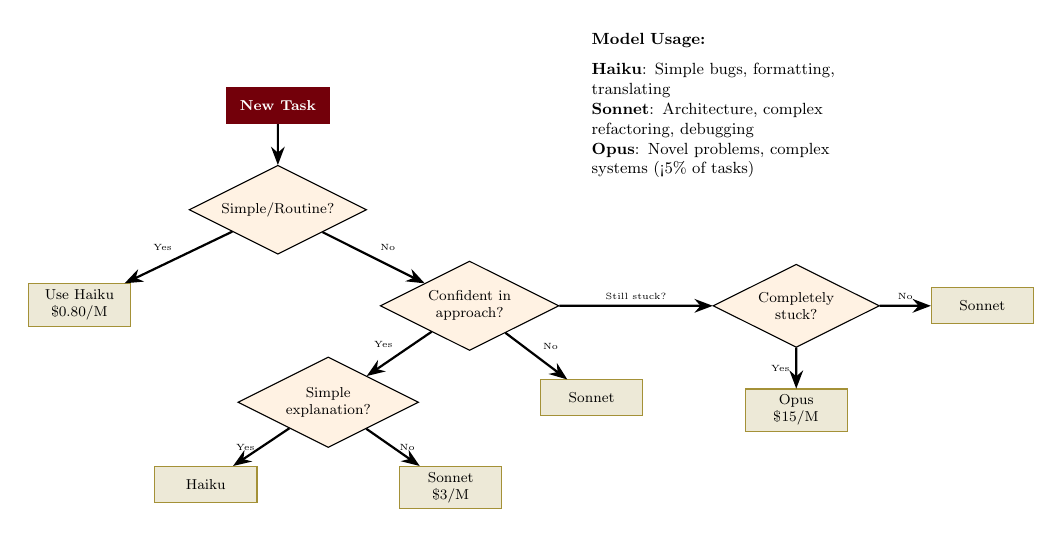
\begin{tikzpicture}[node distance=0.8cm and 1.5cm, scale=0.65, transform shape]
        % Decision tree
        \node (start) [startstop] {New Task};
        \node (q1) [decision, below=of start] {Simple/Routine?};
        \node (haiku1) [cost, below left=1cm and 2cm of q1] {Use Haiku\\\$0.80/M};
        \node (q2) [decision, below right=1cm and 2cm of q1] {Confident in\\approach?};
        \node (q3) [decision, below left=1cm and 1cm of q2] {Simple\\explanation?};
        \node (haiku2) [cost, below left=0.8cm and 0.5cm of q3] {Haiku};
        \node (sonnet1) [cost, below right=0.8cm and 0.5cm of q3] {Sonnet\\\$3/M};
        \node (sonnet2) [cost, below right=1cm and 0.5cm of q2] {Sonnet};
        \node (q4) [decision, right=3cm of q2] {Completely\\stuck?};
        \node (opus) [cost, below=of q4] {Opus\\\$15/M};
        \node (sonnet3) [cost, right=1cm of q4] {Sonnet};

        \draw [arrow] (start) -- (q1);
        \draw [arrow] (q1) -- node[above left, font=\tiny] {Yes} (haiku1);
        \draw [arrow] (q1) -- node[above right, font=\tiny] {No} (q2);
        \draw [arrow] (q2) -- node[above left, font=\tiny] {Yes} (q3);
        \draw [arrow] (q2) -- node[above right, font=\tiny] {No} (sonnet2);
        \draw [arrow] (q3) -- node[left, font=\tiny] {Yes} (haiku2);
        \draw [arrow] (q3) -- node[right, font=\tiny] {No} (sonnet1);
        \draw [arrow] (q2) -- node[above, font=\tiny] {Still stuck?} (q4);
        \draw [arrow] (q4) -- node[left, font=\tiny] {Yes} (opus);
        \draw [arrow] (q4) -- node[above, font=\tiny] {No} (sonnet3);

        % Usage guide
        \node [right=5cm of start, text width=5cm, font=\small] {
            \textbf{Model Usage:}\\[0.2cm]
            \textbf{Haiku}: Simple bugs, formatting, translating\\
            \textbf{Sonnet}: Architecture, complex refactoring, debugging\\
            \textbf{Opus}: Novel problems, complex systems (<5\% of tasks)
        };
    \end{tikzpicture}
\end{frame}

% Slide 23
\begin{frame}[fragile]{Controlling and Planning Agent Costs}
    \textbf{Budget Management Strategies}

    \begin{columns}[T]
        \begin{column}{0.48\textwidth}
            \textbf{Strategy 1: Tiered Budgets}
            \begin{lstlisting}[language=Bash]
Personal learning: $20/month
Production work: $100/month
Research: $50/month
Total: $170/month
Alert if > $200/month
            \end{lstlisting}

            \textbf{Strategy 2: Pre-Commitment}
            \begin{lstlisting}[language=Bash]
"This task might require:
- 3-4 exchanges
- ~30K tokens each
- Model: Sonnet
- Est. cost: $0.50-0.80

Is this within budget? Y/N"
            \end{lstlisting}
        \end{column}
        \begin{column}{0.48\textwidth}
            \textbf{Strategy 3: Rate Limiting}
            \begin{itemize}
                \item "Max 5 agent interactions per day"
                \item Prevents overuse through habit
                \item Forces better planning
            \end{itemize}

            \textbf{Strategy 4: Batch Processing}
            \begin{lstlisting}[language=Bash]
# Bad: 3 separate interactions
Task 1: "Fix lint" - 5K
Task 2: "Fix lint" - 5K
Task 3: "Add comment" - 5K
Total: 15K, 3 interactions

# Good: 1 combined interaction
"Fix these 3 lints and add
this comment" - 12K
Total: 12K, 1 interaction
Savings: 20%
            \end{lstlisting}
        \end{column}
    \end{columns}
\end{frame}

% Slide 24
\begin{frame}{Comparing Costs: Claude Code vs Aider vs Others}
    \textbf{Cost Comparison Across Tools}

    \begin{columns}[T]
        \begin{column}{0.55\textwidth}
            \begin{tabular}{lllr}
                \toprule
                Tool & Model & Cost Model & Typical\\
                \midrule
                Claude Code & Haiku/Sonnet & API pricing & 10-30K\\
                Aider & Haiku/Sonnet & API pricing & Similar\\
                GitHub Copilot & GPT-4 & \$20/month & Per-key\\
                ChatGPT Plus & GPT-4 & \$20/month & Unlimited\\
                Amazon Q & Claude & AWS pricing & Variable\\
                \bottomrule
            \end{tabular}

            \vspace{0.3cm}
            \textbf{Small Bug Fix Cost (\textasciitilde20K tokens):}
            \begin{itemize}
                \item Claude Code (Haiku): \$0.032
                \item ChatGPT Plus: \$0.67 per query avg
            \end{itemize}
        \end{column}
        \begin{column}{0.42\textwidth}
            \textbf{Hybrid Strategy:}

            \begin{block}{Claude Code}
                Specific tasks, occasional use, track costs
            \end{block}

            \begin{block}{ChatGPT Plus}
                Learning, research, quick questions
            \end{block}

            \begin{block}{Copilot}
                Code completion, inline suggestions
            \end{block}

            \textbf{Total: \textasciitilde\$30-50/month}\\
            Coverage: All needs
        \end{column}
    \end{columns}
\end{frame}

% Slide 25
\begin{frame}[fragile]{Pro Tips for Minimizing Agent Costs}
    \textbf{Advanced Cost Optimization}

    \begin{columns}[T]
        \begin{column}{0.48\textwidth}
            \textbf{Tip 1: Use Git, Not Conversation}
            \begin{lstlisting}[language=Bash]
# BAD: Agent outputs all changes
Agent: [Large code output]
Cost: High (all in tokens)

# GOOD: Agent commits directly
Agent: "Done, changes committed"
Cost: Low (minimal output)
            \end{lstlisting}

            \textbf{Tip 2: Reuse Conversation Context}
            \begin{lstlisting}[language=Bash]
# BAD: New conversation each task
Each starts over, no memory

# GOOD: One conversation
"In previous task we did X.
Now do Y."
Savings: 30-50%
            \end{lstlisting}
        \end{column}
        \begin{column}{0.48\textwidth}
            \textbf{Tip 3: Checkpoint and Prune}
            \begin{lstlisting}[language=Bash]
# After major milestone:
git commit -m "Phase 1 complete"

# Start fresh
"We completed auth. Now
build the API layer."
Fresh start: 10K vs 100K
            \end{lstlisting}

            \textbf{Optimized Approach Example:}
            \begin{itemize}
                \item Session 1: Build API (25K)
                \item Session 2: Add auth (15K)
                \item Session 3: Fix bugs (15K)
                \item Session 4: Add tests (15K)
                \item \textbf{Total: 70K = \$0.25}
            \end{itemize}
            vs Naive: 180K = \$0.60\\
            \textbf{Savings: 60\%}
        \end{column}
    \end{columns}
\end{frame}

% Slide 26
\begin{frame}{Should You Use an Agent for This Task?}
    \textbf{ROI and Decision-Making Framework}

    \begin{columns}[T]
        \begin{column}{0.55\textwidth}
            \textbf{Decision Framework:}
            \begin{enumerate}
                \item \textbf{Well-understood task?}\\
                Yes $\rightarrow$ Agent will do well, cheap\\
                No $\rightarrow$ Might be expensive

                \item \textbf{How much planning needed?}\\
                Know what to do $\rightarrow$ Use agent\\
                Need to figure out $\rightarrow$ Plan first

                \item \textbf{What's your time worth?}\\
                High (\$50+/hr) $\rightarrow$ Use agent even if \$0.50\\
                Low (\$15/hr) $\rightarrow$ Only if saves >\$1

                \item \textbf{Learning opportunity?}\\
                Yes $\rightarrow$ Maybe do manually\\
                No $\rightarrow$ Use agent
            \end{enumerate}
        \end{column}
        \begin{column}{0.42\textwidth}
            \textbf{ROI Calculation:}
            \[
            \text{ROI} = (\text{Time saved} \times \text{Rate}) - \text{Cost}
            \]

            \textbf{Example:}
            \begin{itemize}
                \item Task: Refactor auth
                \item Time without agent: 3 hrs
                \item Time with agent: 45 min
                \item Time saved: 2.25 hrs
                \item Rate: \$50/hr
                \item Agent cost: \$0.75
            \end{itemize}

            \textbf{ROI} = (2.25 $\times$ \$50) - \$0.75\\
            = \$112.50 - \$0.75 = \textbf{+\$111.75}

            \begin{block}{Rule of Thumb}
                ROI-positive if saving > 20 min/day
            \end{block}
        \end{column}
    \end{columns}
\end{frame}

% ============================================================
% SECTION 4: TESTING AGENTIC SYSTEMS
% ============================================================
\section{Testing Agentic Systems}

% Slide 27
\begin{frame}{Why Testing Agents is Different}
    \textbf{Challenges of Testing Agent Behavior}

    \begin{columns}[T]
        \begin{column}{0.48\textwidth}
            \textbf{The Challenge:}

            \begin{tabular}{ll}
                \toprule
                Traditional & Agent\\
                \midrule
                Known input & Complex prompt\\
                Deterministic & Variable output\\
                Clear pass/fail & Ambiguous result\\
                \bottomrule
            \end{tabular}

            \vspace{0.3cm}
            \textbf{Non-Determinism:}
            \begin{itemize}
                \item Same prompt, Run 1: Approach A
                \item Same prompt, Run 2: Approach B
                \item Both might be valid!
            \end{itemize}
        \end{column}
        \begin{column}{0.48\textwidth}
            \textbf{Vagueness in Requirements:}
            \begin{itemize}
                \item Traditional: "add(2,3) returns 5"
                \item Agent: "Refactor to be better"
                \begin{itemize}
                    \item Faster?
                    \item More readable?
                    \item More maintainable?
                    \item All of above?
                \end{itemize}
            \end{itemize}

            \vspace{0.3cm}
            \textbf{Cost of Testing:}
            \begin{itemize}
                \item Each test run costs money
                \item 100 runs: \$10-100
                \item Can't run 1000 times
            \end{itemize}

            \begin{alertblock}{Key Insight}
                Different system needs different testing approach.
            \end{alertblock}
        \end{column}
    \end{columns}
\end{frame}

% Slide 28
\begin{frame}{Different Tests for Different Aspects}
    \textbf{Test Categories for Agent Systems}

    \centering
    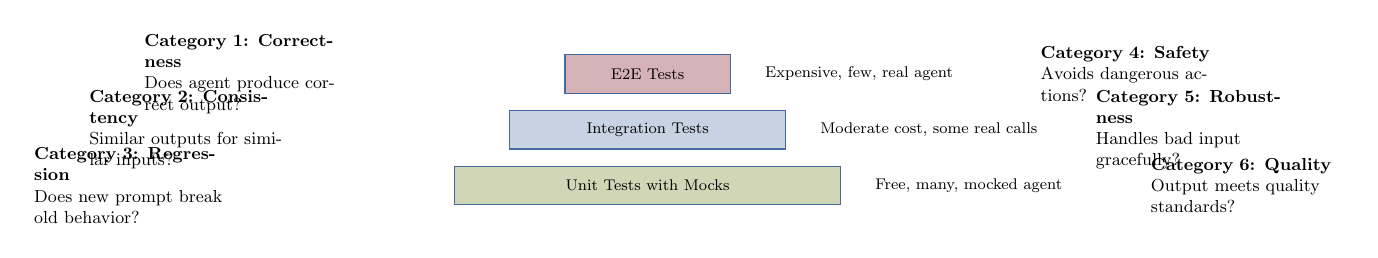
\begin{tikzpicture}[node distance=0.3cm and 0.5cm, scale=0.7, transform shape]
        % Testing Pyramid
        \node (e2e) [test, minimum width=3cm, fill=UofSCGarnet!30] {E2E Tests};
        \node (int) [test, below=of e2e, minimum width=5cm, fill=UofSCAtlantic!30] {Integration Tests};
        \node (unit) [test, below=of int, minimum width=7cm, fill=UofSCHorseshoe!30] {Unit Tests with Mocks};

        % Labels
        \node [right=0.5cm of e2e, font=\footnotesize, text width=4cm] {Expensive, few, real agent};
        \node [right=0.5cm of int, font=\footnotesize, text width=4cm] {Moderate cost, some real calls};
        \node [right=0.5cm of unit, font=\footnotesize, text width=4cm] {Free, many, mocked agent};

        % Categories on left
        \node [left=4cm of e2e, text width=3.5cm, font=\small] {
            \textbf{Category 1: Correctness}\\
            Does agent produce correct output?
        };
        \node [left=4cm of int, text width=3.5cm, font=\small] {
            \textbf{Category 2: Consistency}\\
            Similar outputs for similar inputs?
        };
        \node [left=4cm of unit, text width=3.5cm, font=\small] {
            \textbf{Category 3: Regression}\\
            Does new prompt break old behavior?
        };

        % Right side categories
        \node [right=5.5cm of e2e, text width=3.5cm, font=\small] {
            \textbf{Category 4: Safety}\\
            Avoids dangerous actions?
        };
        \node [right=5.5cm of int, text width=3.5cm, font=\small] {
            \textbf{Category 5: Robustness}\\
            Handles bad input gracefully?
        };
        \node [right=5.5cm of unit, text width=3.5cm, font=\small] {
            \textbf{Category 6: Quality}\\
            Output meets quality standards?
        };
    \end{tikzpicture}
\end{frame}

% Slide 29
\begin{frame}[fragile]{Writing Tests Before Asking Agent}
    \textbf{Test-Driven Development with Agents}

    \begin{columns}[T]
        \begin{column}{0.48\textwidth}
            \textbf{Principle: Define Success Upfront}
            \begin{lstlisting}[language=Python]
# test_auth.py (write BEFORE)

def test_password_hashing():
    from auth import hash_password
    password = "test_password_123"
    hashed = hash_password(password)

    # Verify it's hashed
    assert hashed != password

    # Verify bcrypt format
    assert hashed.startswith("$2")

    # Verify verification works
    assert verify_password(
        password, hashed) == True
    assert verify_password(
        "wrong", hashed) == False
            \end{lstlisting}
        \end{column}
        \begin{column}{0.48\textwidth}
            \textbf{Then show agent the test:}
            \begin{lstlisting}[language=Bash]
"Here's my test suite:
[Tests above]

Please refactor the auth module
to pass these tests.
Run pytest to verify."
            \end{lstlisting}

            \textbf{Agent Response Cycle:}
            \begin{enumerate}
                \item Agent reads tests
                \item Agent attempts refactoring
                \item Agent runs pytest
                \item Tests fail: Agent sees why
                \item Agent fixes issues
                \item Tests pass: Complete!
            \end{enumerate}

            \begin{block}{Benefits}
                Clear criteria, no ambiguity, cost reduction
            \end{block}
        \end{column}
    \end{columns}
\end{frame}

% Slide 30
\begin{frame}[fragile]{Preventing Agent Changes from Breaking Things}
    \textbf{Regression Testing for Agent Workflows}

    \begin{columns}[T]
        \begin{column}{0.48\textwidth}
            \textbf{Baseline Testing Process:}
            \begin{enumerate}
                \item \textbf{Establish baseline}
                \begin{itemize}
                    \item Run current workflow
                    \item Document results
                    \item Save outputs, metrics
                \end{itemize}

                \item \textbf{Make changes}
                \begin{itemize}
                    \item Update prompt/model
                    \item Update parameters
                \end{itemize}

                \item \textbf{Run again}
                \begin{itemize}
                    \item Compare to baseline
                    \item Document differences
                \end{itemize}

                \item \textbf{Regression check}
                \begin{itemize}
                    \item Did new version break anything?
                    \item Any unexpected changes?
                \end{itemize}
            \end{enumerate}
        \end{column}
        \begin{column}{0.48\textwidth}
            \textbf{Version Comparison:}

            \begin{tabular}{lrrr}
                \toprule
                Metric & V1 & V2 & Change\\
                \midrule
                Success rate & 95\% & 92\% & -3\%\\
                Avg tokens & 25K & 24K & -1K\\
                Avg time & 2m & 2.5m & +30s\\
                Quality & 8/10 & 8.2/10 & +0.2\\
                Test pass & 98\% & 99\% & +1\%\\
                \bottomrule
            \end{tabular}

            \textbf{Regression detected?} No significant regressions\\
            \textbf{Decision:} Deploy version 2

            \begin{block}{Continuous Regression}
                Run on each commit. Alert if any metric drops >5\%.
            \end{block}
        \end{column}
    \end{columns}
\end{frame}

% Slide 31
\begin{frame}[fragile]{How to Know if Agent Output is Good}
    \textbf{Validating Agent Output Quality}

    \begin{columns}[T]
        \begin{column}{0.48\textwidth}
            \textbf{Quality Dimensions:}

            \begin{tabular}{lr}
                \toprule
                Dimension & Points\\
                \midrule
                Correctness & 0-30\\
                Readability & 0-20\\
                Documentation & 0-20\\
                Security & 0-20\\
                Performance & 0-10\\
                \midrule
                \textbf{Total} & \textbf{0-100}\\
                \bottomrule
            \end{tabular}

            \vspace{0.3cm}
            \textbf{Acceptance Criteria:}
            \begin{itemize}
                \item 0-39: Not acceptable, redo
                \item 40-69: Acceptable with fixes
                \item 70-84: Good quality
                \item 85-100: Excellent, production-ready
            \end{itemize}
        \end{column}
        \begin{column}{0.48\textwidth}
            \textbf{Scoring Example:}
            \begin{lstlisting}[language=Python]
def total_score(code):
    return sum([
        correctness(),  # Tests pass?
        readability(),  # Clear names?
        documentation(), # Docstrings?
        security(),     # No vulns?
        performance()   # Efficient?
    ])
            \end{lstlisting}

            \textbf{Manual Review Checklist:}
            \begin{itemize}
                \item[$\square$] Does it actually work?
                \item[$\square$] Are variable names clear?
                \item[$\square$] Any security issues?
                \item[$\square$] Any performance issues?
                \item[$\square$] Tests added/updated?
                \item[$\square$] Documentation updated?
            \end{itemize}
        \end{column}
    \end{columns}
\end{frame}

% Slide 32
\begin{frame}[fragile]{Testing Agents Without Running Expensive Operations}
    \textbf{Mocking and Simulation for Agent Testing}

    \begin{columns}[T]
        \begin{column}{0.48\textwidth}
            \textbf{Mock the Agent:}
            \begin{lstlisting}[language=Python]
from unittest.mock import Mock, patch

def test_workflow_with_mock():
    # Create mock agent
    mock_agent = Mock()
    mock_agent.analyze_code.return_value = {
        "issues": ["SQL injection"],
        "severity": "HIGH"
    }

    # Patch real agent with mock
    with patch('mycode.agent',
               mock_agent):
        result = run_workflow(code)

        assert result["issues"] == 1
        assert result["severity"] == "HIGH"
            \end{lstlisting}
        \end{column}
        \begin{column}{0.48\textwidth}
            \textbf{Cost Comparison:}

            \begin{tabular}{lrr}
                \toprule
                Approach & Tests & Cost\\
                \midrule
                Mock testing & 1000 & \$0\\
                Real agent & 10 & \$0.50-1\\
                \bottomrule
            \end{tabular}

            \vspace{0.3cm}
            \textbf{Best Practice:}
            \begin{itemize}
                \item Use mocks for 99\% of tests
                \item Use real agent for 1\% critical tests
            \end{itemize}

            \textbf{Simulate Different Behaviors:}
            \begin{itemize}
                \item Agent success
                \item Agent failure
                \item Agent timeout
                \item Agent hallucination
            \end{itemize}
        \end{column}
    \end{columns}
\end{frame}

% Slide 33
\begin{frame}{Automated Testing in CI/CD Pipelines}
    \textbf{Continuous Integration for Agent Workflows}

    \centering
    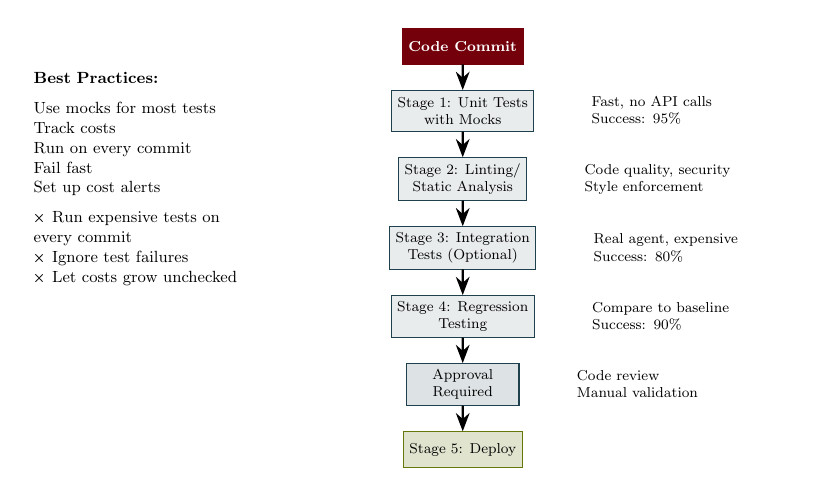
\begin{tikzpicture}[node distance=0.5cm and 0.8cm, scale=0.65, transform shape]
        % Pipeline stages
        \node (commit) [startstop] {Code Commit};
        \node (unit) [pipeline, below=of commit] {Stage 1: Unit Tests\\with Mocks};
        \node (lint) [pipeline, below=of unit] {Stage 2: Linting/\\Static Analysis};
        \node (int) [pipeline, below=of lint] {Stage 3: Integration\\Tests (Optional)};
        \node (reg) [pipeline, below=of int] {Stage 4: Regression\\Testing};
        \node (approve) [human, below=of reg] {Approval\\Required};
        \node (deploy) [success, below=of approve] {Stage 5: Deploy};

        \draw [arrow] (commit) -- (unit);
        \draw [arrow] (unit) -- (lint);
        \draw [arrow] (lint) -- (int);
        \draw [arrow] (int) -- (reg);
        \draw [arrow] (reg) -- (approve);
        \draw [arrow] (approve) -- (deploy);

        % Properties
        \node [right=1cm of unit, font=\footnotesize, text width=4cm] {Fast, no API calls\\Success: 95\%};
        \node [right=1cm of lint, font=\footnotesize, text width=4cm] {Code quality, security\\Style enforcement};
        \node [right=1cm of int, font=\footnotesize, text width=4cm] {Real agent, expensive\\Success: 80\%};
        \node [right=1cm of reg, font=\footnotesize, text width=4cm] {Compare to baseline\\Success: 90\%};
        \node [right=1cm of approve, font=\footnotesize, text width=4cm] {Code review\\Manual validation};

        % Best practices
        \node [left=3cm of lint, text width=4cm, font=\small] {
            \textbf{Best Practices:}\\[0.2cm]
            \checkmark{} Use mocks for most tests\\
            \checkmark{} Track costs\\
            \checkmark{} Run on every commit\\
            \checkmark{} Fail fast\\
            \checkmark{} Set up cost alerts\\[0.2cm]
            \texttimes{} Run expensive tests on every commit\\
            \texttimes{} Ignore test failures\\
            \texttimes{} Let costs grow unchecked
        };
    \end{tikzpicture}
\end{frame}

% Slide 34
\begin{frame}{Tracking Agent Behavior Over Time}
    \textbf{Monitoring and Observability in Production}

    \begin{columns}[T]
        \begin{column}{0.48\textwidth}
            \textbf{What to Monitor:}

            \begin{block}{Availability}
                Agent online/offline, API response time, error rates
            \end{block}

            \begin{block}{Quality}
                Task success rate, output quality scores, user satisfaction
            \end{block}

            \begin{block}{Cost}
                Tokens per task, total costs trending, cost per successful task
            \end{block}

            \begin{block}{Performance}
                Time per task, token efficiency, model selection efficiency
            \end{block}
        \end{column}
        \begin{column}{0.48\textwidth}
            \textbf{Dashboard Views:}
            \begin{enumerate}
                \item \textbf{Real-time status}\\
                Current task, API health, errors (1hr)

                \item \textbf{Daily trends}\\
                Success rate, avg tokens, cost, quality

                \item \textbf{Weekly summary}\\
                Total tasks, common errors, trends
            \end{enumerate}

            \vspace{0.3cm}
            \textbf{Alerts:}
            \begin{itemize}
                \item Success rate < 80\%
                \item Cost per task increases 20\%+
                \item Quality score < 6/10
                \item API error rate > 5\%
            \end{itemize}
        \end{column}
    \end{columns}
\end{frame}

% ============================================================
% SECTION 5: INTEGRATION PATTERNS
% ============================================================
\section{Integration Patterns}

% Slide 35
\begin{frame}{Agents as Part of Your Development Workflow}
    \textbf{Combining Agents with CI/CD Pipelines}

    \centering
    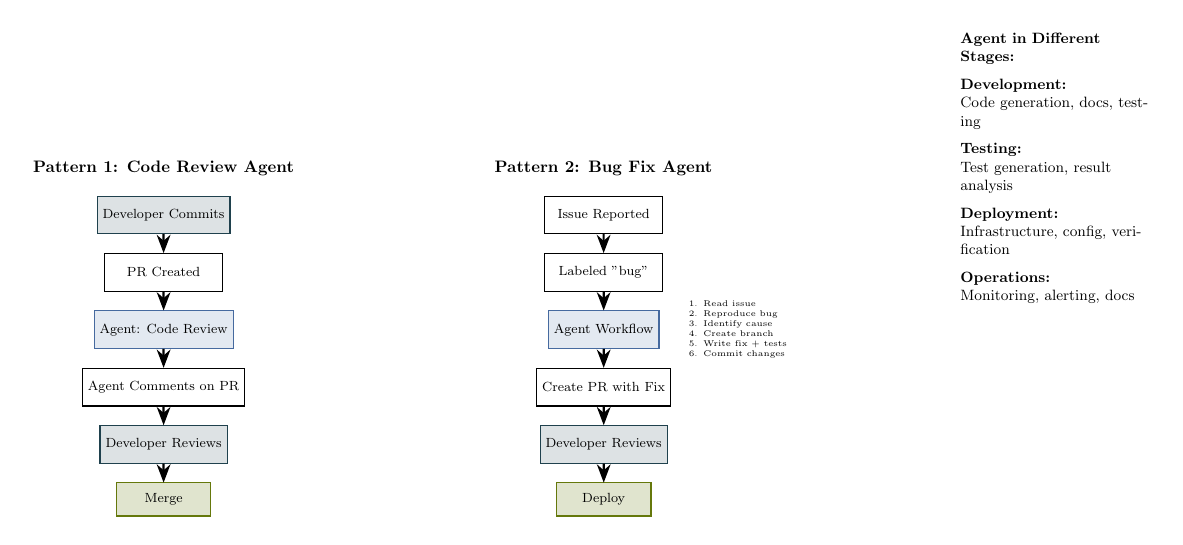
\begin{tikzpicture}[node distance=0.4cm and 1cm, scale=0.6, transform shape]
        % Code Review Agent Pattern
        \node (title1) [font=\bfseries] {Pattern 1: Code Review Agent};
        \node (dev) [human, below=0.3cm of title1] {Developer Commits};
        \node (pr) [process, below=of dev] {PR Created};
        \node (agent1) [agent, below=of pr] {Agent: Code Review};
        \node (comment) [process, below=of agent1] {Agent Comments on PR};
        \node (review) [human, below=of comment] {Developer Reviews};
        \node (merge) [success, below=of review] {Merge};

        \draw [arrow] (dev) -- (pr);
        \draw [arrow] (pr) -- (agent1);
        \draw [arrow] (agent1) -- (comment);
        \draw [arrow] (comment) -- (review);
        \draw [arrow] (review) -- (merge);

        % Bug Fix Agent Pattern
        \node (title2) [font=\bfseries, right=4cm of title1] {Pattern 2: Bug Fix Agent};
        \node (issue) [process, below=0.3cm of title2] {Issue Reported};
        \node (label) [process, below=of issue] {Labeled "bug"};
        \node (agent2) [agent, below=of label] {Agent Workflow};
        \node (fix) [process, below=of agent2] {Create PR with Fix};
        \node (dev2) [human, below=of fix] {Developer Reviews};
        \node (deploy) [success, below=of dev2] {Deploy};

        \draw [arrow] (issue) -- (label);
        \draw [arrow] (label) -- (agent2);
        \draw [arrow] (agent2) -- (fix);
        \draw [arrow] (fix) -- (dev2);
        \draw [arrow] (dev2) -- (deploy);

        % Agent workflow details
        \node [right=0.5cm of agent2, font=\tiny, text width=2.5cm] {
            1. Read issue\\
            2. Reproduce bug\\
            3. Identify cause\\
            4. Create branch\\
            5. Write fix + tests\\
            6. Commit changes
        };

        % Agent stages
        \node [right=5cm of title2, text width=4cm, font=\small] {
            \textbf{Agent in Different Stages:}\\[0.2cm]
            \textbf{Development:}\\
            Code generation, docs, testing\\[0.2cm]
            \textbf{Testing:}\\
            Test generation, result analysis\\[0.2cm]
            \textbf{Deployment:}\\
            Infrastructure, config, verification\\[0.2cm]
            \textbf{Operations:}\\
            Monitoring, alerting, docs
        };
    \end{tikzpicture}
\end{frame}

% Slide 36
\begin{frame}{Collaboration Patterns When Teams Use Agents}
    \textbf{Using Agents in Team Workflows}

    \begin{columns}[T]
        \begin{column}{0.48\textwidth}
            \textbf{Pattern 1: Shared Agent Prompts}
            \begin{itemize}
                \item Team maintains: agent-prompts/
                \item code-review.md
                \item refactoring.md
                \item documentation.md
                \item Same prompts $\rightarrow$ consistent results
            \end{itemize}

            \vspace{0.3cm}
            \textbf{Pattern 2: Agent Guardrails}
            \begin{itemize}
                \item \textbf{Can:} read, analyze, suggest
                \item \textbf{Cannot:} commit, push, deploy without approval
                \item \textbf{Must:} provide clear explanations
                \item \textbf{Should:} flag security issues
            \end{itemize}
        \end{column}
        \begin{column}{0.48\textwidth}
            \textbf{Pattern 3: Agent Results Review}
            \begin{enumerate}
                \item Agent generates code
                \item Team reviews output
                \item Humans decide: accept, modify, reject
            \end{enumerate}
            \textbf{Never:} "Just run agent and deploy"

            \vspace{0.3cm}
            \textbf{Team Onboarding:}
            \begin{enumerate}
                \item How agents work (capabilities/limits)
                \item Team agent usage policy
                \item Standard prompts
                \item How to review agent output
                \item What to do if something goes wrong
            \end{enumerate}

            \textit{Autonomy after 5-10 supervised tasks}
        \end{column}
    \end{columns}
\end{frame}

% Slide 37
\begin{frame}[fragile]{Managing Code and Workflows Under Source Control}
    \textbf{Version Control Best Practices with Agents}

    \begin{columns}[T]
        \begin{column}{0.48\textwidth}
            \textbf{Good Git Practices:}
            \begin{lstlisting}[language=Bash]
# Commit frequently
git add auth.py
git commit -m "refactor: extract
password validation method"

# Before agent work
git checkout -b feature/auth

# Agent makes changes
# 1. Read code
# 2. Make changes
# 3. Run tests
# 4. Commit

# After verification
git push origin feature/auth
# Create Pull Request
            \end{lstlisting}
        \end{column}
        \begin{column}{0.48\textwidth}
            \textbf{Conventional Commits:}
            \begin{lstlisting}[language=Bash]
<type>: <description>

Types:
- feat: new feature
- fix: bug fix
- refactor: code reorg
- test: tests only
- docs: documentation
- perf: performance

Examples:
feat: add OAuth 2.0 support
fix: prevent SQL injection
refactor: simplify auth flow
            \end{lstlisting}

            \textbf{Useful Commands:}
            \begin{itemize}
                \item git diff HEAD (see changes)
                \item git log -p auth.py (file history)
                \item git tag backup-before-refactor
            \end{itemize}
        \end{column}
    \end{columns}
\end{frame}

% Slide 38
\begin{frame}{Agents as Code Reviewers and Assistants}
    \textbf{Code Review Integration}

    \begin{columns}[T]
        \begin{column}{0.48\textwidth}
            \textbf{Scenario 1: Agent Reviews Human Code}
            \begin{enumerate}
                \item Developer submits PR
                \item Agent analyzes for:
                \begin{itemize}
                    \item Security issues
                    \item Performance problems
                    \item Style violations
                    \item Missing tests
                    \item Potential bugs
                \end{itemize}
                \item Agent comments on PR
                \item Human reviewer makes final decision
            \end{enumerate}
        \end{column}
        \begin{column}{0.48\textwidth}
            \textbf{Scenario 2: Human Reviews Agent Code}
            \begin{enumerate}
                \item Agent generates code
                \item Human reviews for:
                \begin{itemize}
                    \item Requirements match?
                    \item Quality acceptable?
                    \item Edge cases covered?
                    \item Design sound?
                \end{itemize}
                \item Decision: approve, modify, reject
            \end{enumerate}

            \vspace{0.3cm}
            \textbf{Automated Tools (use alongside):}
            \begin{itemize}
                \item Linting: eslint, pylint, clippy
                \item Security: bandit, sqlmap
                \item Type checking: mypy, TypeScript
            \end{itemize}
        \end{column}
    \end{columns}
\end{frame}

% Slide 39
\begin{frame}[fragile]{Using Agents to Automate Terminal Workflows}
    \textbf{Scripting and Terminal Automation}

    \begin{columns}[T]
        \begin{column}{0.48\textwidth}
            \textbf{Scenario 1: Batch File Processing}
            \begin{lstlisting}[language=Bash]
# Agent-assisted approach:
"Write a script that:
- Reads all files in logs/
- Extracts ERROR or CRITICAL
- Aggregates into report.md
- Groups by error type
- Provides count and sample"

# Agent writes script
# You verify and run
# Result: 100 files in seconds
            \end{lstlisting}

            \textbf{Scenario 2: Testing Automation}
            \begin{lstlisting}[language=Bash]
# Agent creates: run_tests.sh
echo "Running unit tests..."
pytest tests/unit/ -v --cov
echo "Running integration..."
pytest tests/integration/ -v
echo "Generating coverage..."
coverage html
            \end{lstlisting}
        \end{column}
        \begin{column}{0.48\textwidth}
            \textbf{Scenario 3: Deployment}
            \begin{lstlisting}[language=Bash]
# Agent creates: deploy.sh
#!/bin/bash
set -e

echo "Pre-deployment checks..."
./scripts/pre-deploy.sh

echo "Running tests..."
npm run test

echo "Building..."
npm run build

echo "Creating backup..."
git tag "backup-$(date +%Y%m%d)"

echo "Deploying..."
docker build -t app:latest .
docker push app:latest

echo "Deployment complete!"
            \end{lstlisting}

            \textbf{Benefits:} Time savings, error reduction, self-documentation
        \end{column}
    \end{columns}
\end{frame}

% Slide 40
\begin{frame}{Building a Complete Agentic Workflow}
    \textbf{Real-World Integration Example}

    \centering
    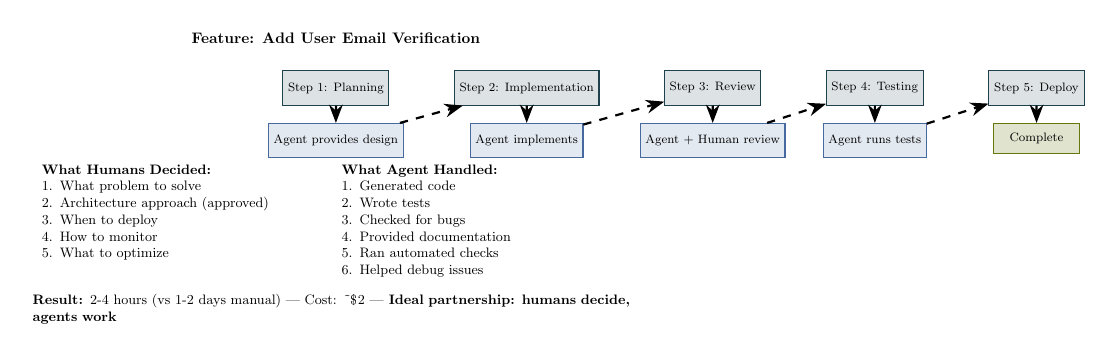
\begin{tikzpicture}[node distance=0.4cm and 0.8cm, scale=0.55, transform shape]
        % Timeline
        \node (title) [font=\bfseries] {Feature: Add User Email Verification};

        \node (step1) [human, below=0.5cm of title] {Step 1: Planning};
        \node (a1) [agent, below=of step1] {Agent provides design};

        \node (step2) [human, right=1.5cm of step1] {Step 2: Implementation};
        \node (a2) [agent, below=of step2] {Agent implements};

        \node (step3) [human, right=1.5cm of step2] {Step 3: Review};
        \node (a3) [agent, below=of step3] {Agent + Human review};

        \node (step4) [human, right=1.5cm of step3] {Step 4: Testing};
        \node (a4) [agent, below=of step4] {Agent runs tests};

        \node (step5) [human, right=1.5cm of step4] {Step 5: Deploy};
        \node (a5) [success, below=of step5] {Complete};

        \draw [arrow] (step1) -- (a1);
        \draw [arrow] (step2) -- (a2);
        \draw [arrow] (step3) -- (a3);
        \draw [arrow] (step4) -- (a4);
        \draw [arrow] (step5) -- (a5);

        \draw [arrow, dashed] (a1) -- (step2);
        \draw [arrow, dashed] (a2) -- (step3);
        \draw [arrow, dashed] (a3) -- (step4);
        \draw [arrow, dashed] (a4) -- (step5);

        % Details below
        \node [below=2.5cm of title, text width=14cm, font=\small] {
            \begin{tabular}{p{6.5cm}p{6.5cm}}
                \textbf{What Humans Decided:} & \textbf{What Agent Handled:}\\
                1. What problem to solve & 1. Generated code\\
                2. Architecture approach (approved) & 2. Wrote tests\\
                3. When to deploy & 3. Checked for bugs\\
                4. How to monitor & 4. Provided documentation\\
                5. What to optimize & 5. Ran automated checks\\
                & 6. Helped debug issues\\
            \end{tabular}

            \vspace{0.3cm}
            \textbf{Result:} 2-4 hours (vs 1-2 days manual) | Cost: \textasciitilde\$2 | \textbf{Ideal partnership: humans decide, agents work}
        };
    \end{tikzpicture}
\end{frame}

% ============================================================
% SECTION 6: REAL-WORLD CASE STUDIES & CONCLUSION
% ============================================================
\section{Real-World Case Studies \& Conclusion}

% Slide 41
\begin{frame}{How Agents Accelerated a Startup MVP}
    \textbf{Success Case Study - Rapid Prototyping}

    \centering
    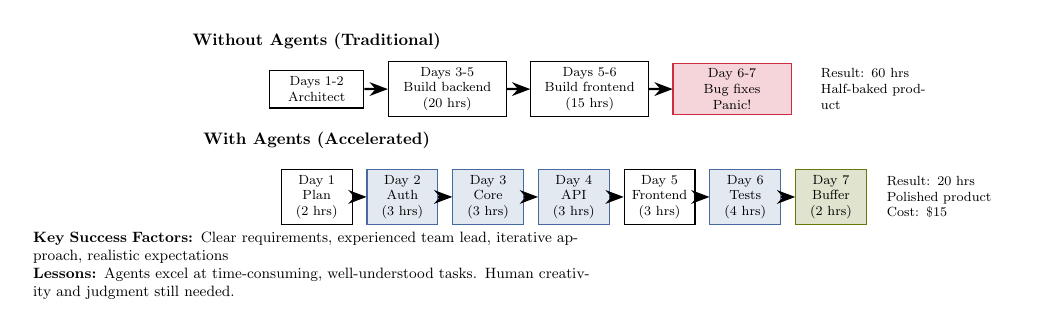
\begin{tikzpicture}[node distance=0.3cm and 1cm, scale=0.6, transform shape]
        % Timeline comparison
        \node (title1) [font=\bfseries] {Without Agents (Traditional)};
        \node (d1) [process, below=0.3cm of title1, minimum width=2cm] {Days 1-2\\Architect};
        \node (d2) [process, right=0.5cm of d1, minimum width=2.5cm] {Days 3-5\\Build backend\\(20 hrs)};
        \node (d3) [process, right=0.5cm of d2, minimum width=2.5cm] {Days 5-6\\Build frontend\\(15 hrs)};
        \node (d4) [failure, right=0.5cm of d3, minimum width=2.5cm] {Day 6-7\\Bug fixes\\Panic!};

        \draw [arrow] (d1) -- (d2);
        \draw [arrow] (d2) -- (d3);
        \draw [arrow] (d3) -- (d4);

        \node [right=0.5cm of d4, font=\footnotesize, text width=2.5cm] {Result: 60 hrs\\Half-baked product};

        % With agents
        \node (title2) [font=\bfseries, below=1.5cm of title1] {With Agents (Accelerated)};
        \node (a1) [process, below=0.3cm of title2, minimum width=1.5cm] {Day 1\\Plan\\(2 hrs)};
        \node (a2) [agent, right=0.3cm of a1, minimum width=1.5cm] {Day 2\\Auth\\(3 hrs)};
        \node (a3) [agent, right=0.3cm of a2, minimum width=1.5cm] {Day 3\\Core\\(3 hrs)};
        \node (a4) [agent, right=0.3cm of a3, minimum width=1.5cm] {Day 4\\API\\(3 hrs)};
        \node (a5) [process, right=0.3cm of a4, minimum width=1.5cm] {Day 5\\Frontend\\(3 hrs)};
        \node (a6) [agent, right=0.3cm of a5, minimum width=1.5cm] {Day 6\\Tests\\(4 hrs)};
        \node (a7) [success, right=0.3cm of a6, minimum width=1.5cm] {Day 7\\Buffer\\(2 hrs)};

        \draw [arrow] (a1) -- (a2);
        \draw [arrow] (a2) -- (a3);
        \draw [arrow] (a3) -- (a4);
        \draw [arrow] (a4) -- (a5);
        \draw [arrow] (a5) -- (a6);
        \draw [arrow] (a6) -- (a7);

        \node [right=0.3cm of a7, font=\footnotesize, text width=2.5cm] {Result: 20 hrs\\Polished product\\Cost: \$15};

        % Key factors
        \node [below=1.5cm of title2, text width=12cm, font=\small] {
            \textbf{Key Success Factors:} Clear requirements, experienced team lead, iterative approach, realistic expectations\\
            \textbf{Lessons:} Agents excel at time-consuming, well-understood tasks. Human creativity and judgment still needed.
        };
    \end{tikzpicture}
\end{frame}

% Slide 42
\begin{frame}{When Relying Too Much on Agents Goes Wrong}
    \textbf{Failure Case Study - Over-Automation}

    \begin{columns}[T]
        \begin{column}{0.48\textwidth}
            \textbf{The Problems:}

            \textbf{Week 1:} "Agent generated code, we deployed"
            \begin{itemize}
                \item[\textcolor{UofSCRose}{\texttimes}] Security vulnerability in production
                \item[\textcolor{UofSCRose}{\texttimes}] Customer data exposed
                \item Root cause: No code review before deploy
            \end{itemize}

            \textbf{Week 2:} "Use agent for all code"
            \begin{itemize}
                \item[\textcolor{UofSCRose}{\texttimes}] Token costs skyrocket
                \item[\textcolor{UofSCRose}{\texttimes}] \$500/month vs \$50 planned
                \item Root cause: No optimization
            \end{itemize}

            \textbf{Week 3:} "Agent refactored wrong part"
            \begin{itemize}
                \item[\textcolor{UofSCRose}{\texttimes}] Broke critical functionality
                \item Root cause: Vague instruction
            \end{itemize}
        \end{column}
        \begin{column}{0.48\textwidth}
            \textbf{What Went Wrong:}
            \begin{enumerate}
                \item No code review process
                \item Over-trust in agent capability
                \item No budget management
                \item Vague requirements
                \item No testing before deploy
            \end{enumerate}

            \vspace{0.3cm}
            \textbf{Recovery (Month 2-3):}
            \begin{itemize}
                \item Implement mandatory code review
                \item Define agent use cases explicitly
                \item Set budget limits
                \item Improve prompt clarity
                \item Gradually re-adopt with guardrails
            \end{itemize}

            \begin{alertblock}{Lesson}
                Agents need proper governance. They're not magic - they're tools.
            \end{alertblock}
        \end{column}
    \end{columns}
\end{frame}

% Slide 43
\begin{frame}{Recognizing Limitations and Boundaries}
    \textbf{When NOT to Use Agents}

    \begin{columns}[T]
        \begin{column}{0.48\textwidth}
            \textbf{Don't Use Agents For:}

            \begin{enumerate}
                \item \textbf{Strategic Decisions}\\
                Agent can analyze, human must decide

                \item \textbf{Exploratory Research}\\
                If goal is understanding, do it yourself

                \item \textbf{New Problem Domains}\\
                Learning is necessary

                \item \textbf{High-Risk Systems}\\
                Medical, financial need expert review

                \item \textbf{One-Time Complex Tasks}\\
                Setup overhead > time saved

                \item \textbf{When Speed Isn't Important}\\
                No time pressure = no urgency for agents
            \end{enumerate}
        \end{column}
        \begin{column}{0.48\textwidth}
            \textbf{When to Avoid:}

            \begin{block}{No Time for Learning Curve}
                10 hrs to learn agents, task takes 5 hrs\\
                $\rightarrow$ Might not be worth it
            \end{block}

            \begin{block}{No Verification Capability}
                Can't tell if output is correct\\
                $\rightarrow$ Risky to use agent
            \end{block}

            \begin{block}{Security Concern}
                Sensitive code, credentials present\\
                $\rightarrow$ Risk > benefit
            \end{block}

            \begin{block}{Cultural Resistance}
                Team doesn't trust automation\\
                $\rightarrow$ Resistance will sink adoption
            \end{block}
        \end{column}
    \end{columns}
\end{frame}

% Slide 44
\begin{frame}{Ideal Use Cases for Maximum Value}
    \textbf{When Agents Shine}

    \begin{columns}[T]
        \begin{column}{0.48\textwidth}
            \textbf{1. Well-Understood Problems}
            \begin{itemize}
                \item Common, documented patterns
                \item Clear requirements
                \item Examples: REST APIs, CRUD, refactoring
            \end{itemize}

            \textbf{2. Time-Consuming, Repetitive Work}
            \begin{itemize}
                \item Lots of boilerplate code
                \item Humans find tedious
                \item Examples: tests, migrations, configs
            \end{itemize}

            \textbf{3. Exploratory and Prototyping}
            \begin{itemize}
                \item Quick experimentation
                \item Low cost of being wrong
                \item Examples: MVPs, POCs, spikes
            \end{itemize}
        \end{column}
        \begin{column}{0.48\textwidth}
            \textbf{4. Review and Analysis}
            \begin{itemize}
                \item Comprehensive, consistent reviews
                \item Examples: code review, docs, coverage
            \end{itemize}

            \textbf{5. Context Gathering \& Docs}
            \begin{itemize}
                \item Summarizing large codebases
                \item Examples: README, API docs
            \end{itemize}

            \textbf{6. Skill-Building \& Learning}
            \begin{itemize}
                \item Agent provides examples
                \item You learn by reviewing
            \end{itemize}

            \begin{block}{Success Indicators}
                Well-understood, clear requirements, can verify, time saved, cost reasonable, risk acceptable
            \end{block}
        \end{column}
    \end{columns}
\end{frame}

% Slide 45
\begin{frame}{Where Agentic Tools Are Headed}
    \textbf{Future Directions and Evolution}

    \begin{columns}[T]
        \begin{column}{0.32\textwidth}
            \textbf{Near-term (6-12 months):}
            \begin{itemize}
                \item Better specialization
                \item Improved reliability
                \item Less hallucination
                \item Better integration
                \item Cost reduction
            \end{itemize}
        \end{column}
        \begin{column}{0.32\textwidth}
            \textbf{Medium-term (1-2 years):}
            \begin{itemize}
                \item Autonomous agents
                \item Better reasoning
                \item Multi-step workflows
                \item Team collaboration
                \item Multiple agents working together
            \end{itemize}
        \end{column}
        \begin{column}{0.32\textwidth}
            \textbf{Long-term (2+ years):}
            \begin{itemize}
                \item Agents as colleagues
                \item Continuous improvement
                \item Natural language interfaces
                \item Cross-domain reasoning
            \end{itemize}

            \vspace{0.3cm}
            \textbf{Challenges:}
            \begin{itemize}
                \item Safety at scale
                \item Cost efficiency
                \item Environmental impact
                \item Regulatory compliance
            \end{itemize}
        \end{column}
    \end{columns}

    \vspace{0.4cm}
    \begin{block}{How to Stay Current}
        Follow development (HN, Twitter), join communities (Discord, Reddit), experiment with new tools, share learnings
    \end{block}
\end{frame}

% Slide 46
\begin{frame}{How to Become Expert in Using Agents}
    \textbf{Building Your Agent Mastery}

    \begin{columns}[T]
        \begin{column}{0.32\textwidth}
            \textbf{Phase 1: Fundamentals}\\
            (Weeks 1-4) \textcolor{UofSCHorseshoe}{\checkmark{} Completed!}
            \begin{itemize}
                \item Understand capabilities/limits
                \item Learn clear prompts
                \item Practice terminal usage
                \item Understand cost model
            \end{itemize}

            \textit{Result: Use agents for simple tasks}
        \end{column}
        \begin{column}{0.32\textwidth}
            \textbf{Phase 2: Intermediate}\\
            (Months 2-3)
            \begin{itemize}
                \item Optimize prompts
                \item Build complete workflows
                \item Integrate with CI/CD
                \item Handle failures gracefully
                \item Mentor others
            \end{itemize}

            \textit{Result: Use agents for complex tasks}
        \end{column}
        \begin{column}{0.32\textwidth}
            \textbf{Phase 3: Expert}\\
            (Months 4+)
            \begin{itemize}
                \item Design agent workflows
                \item Optimize organization-wide
                \item Establish best practices
                \item Innovate new patterns
                \item Contribute to open source
            \end{itemize}

            \textit{Result: Thought leader}
        \end{column}
    \end{columns}

    \vspace{0.4cm}
    \begin{block}{Your Next Steps}
        Week 1: Complete activities | Weeks 2-4: Use on real projects | Month 2: Tackle complex tasks | Month 3: Build complete system
    \end{block}
\end{frame}

% Slide 47
\begin{frame}{Distilled Wisdom from Part 8}
    \textbf{Key Takeaways and Principles}

    \begin{columns}[T]
        \begin{column}{0.48\textwidth}
            \textbf{Principle 1: Tools, Not Magic}\\
            Right tool for right job. Be selective.

            \vspace{0.2cm}
            \textbf{Principle 2: Failures Are Learning}\\
            Each failure teaches something. Document and share.

            \vspace{0.2cm}
            \textbf{Principle 3: Clarity Beats Sophistication}\\
            Clear, simple prompts work best.

            \vspace{0.2cm}
            \textbf{Principle 4: Verification Always Required}\\
            Agents make mistakes. Review and test.
        \end{column}
        \begin{column}{0.48\textwidth}
            \textbf{Principle 5: Cost Awareness Matters}\\
            Track spending, optimize queries, budget.

            \vspace{0.2cm}
            \textbf{Principle 6: Security is Your Responsibility}\\
            Set boundaries, restrict access, rotate credentials.

            \vspace{0.2cm}
            \textbf{Principle 7: Human-Agent Partnership}\\
            Humans decide, agents work, humans verify.

            \vspace{0.2cm}
            \textbf{Principle 8: Continuous Improvement}\\
            Iterate, learn, update, share.
        \end{column}
    \end{columns}

    \vspace{0.4cm}
    \begin{block}{These Principles Transcend Specific Tools}
        Whether using Claude Code, Aider, or tools not yet invented---these principles will serve you well.
    \end{block}
\end{frame}

% Slide 48
\begin{frame}{Mindset for Working with Agents}
    \textbf{Final Thoughts: Agent Development Ethos}

    \begin{columns}[T]
        \begin{column}{0.48\textwidth}
            \textbf{Collaborative Mindset:}
            \begin{itemize}
                \item Think of agent as junior colleague
                \item Not: "Make it work"
                \item Think: "Here's what I need, can you help?"
            \end{itemize}

            \vspace{0.3cm}
            \textbf{Humble Approach:}
            \begin{itemize}
                \item You might misunderstand
                \item Agent might misunderstand
                \item Misunderstandings are normal
                \item Iteration is expected
            \end{itemize}
        \end{column}
        \begin{column}{0.48\textwidth}
            \textbf{Experimentation Culture:}
            \begin{itemize}
                \item Try different prompts
                \item Experiment with approaches
                \item Document findings
                \item Share learnings
            \end{itemize}

            \vspace{0.3cm}
            \textbf{Ethical Responsibility:}
            \begin{itemize}
                \item Agents are powerful
                \item Power brings responsibility
                \item Use to create value
                \item Never use to harm
            \end{itemize}
        \end{column}
    \end{columns}

    \vspace{0.4cm}
    \begin{block}{The Excitement of This Era}
        Agent technology is rapidly advancing. Adoption is just beginning. Rules are still being written. You'll help shape how this evolves.
    \end{block}
\end{frame}

% Slide 49
\begin{frame}{Where to Learn More}
    \textbf{Resources and Further Reading}

    \begin{columns}[T]
        \begin{column}{0.32\textwidth}
            \textbf{Official Documentation:}
            \begin{itemize}
                \item anthropic.com/research
                \item docs.anthropic.com
                \item Claude API docs
                \item Aider GitHub
            \end{itemize}

            \vspace{0.3cm}
            \textbf{Key Papers:}
            \begin{itemize}
                \item "Attention is All You Need"
                \item "Chain-of-Thought Prompting"
                \item "ReAct" paper
                \item "Constitutional AI"
            \end{itemize}
        \end{column}
        \begin{column}{0.32\textwidth}
            \textbf{Learning Resources:}
            \begin{itemize}
                \item Deeplearning.AI courses
                \item Fast.ai NLP courses
                \item Andrew Ng's ML courses
            \end{itemize}

            \vspace{0.3cm}
            \textbf{Communities:}
            \begin{itemize}
                \item Hugging Face community
                \item Papers With Code
                \item Local AI/ML meetups
                \item University AI clubs
            \end{itemize}
        \end{column}
        \begin{column}{0.32\textwidth}
            \textbf{Tools to Explore:}
            \begin{itemize}
                \item Langchain (frameworks)
                \item LlamaIndex (indexing)
                \item Hugging Face (models)
                \item Cursor (IDE)
                \item Continue.dev (plugin)
            \end{itemize}

            \vspace{0.3cm}
            \textbf{Staying Updated:}
            \begin{itemize}
                \item Anthropic newsletters
                \item The Batch
                \item AI podcasts
                \item Twitter/X AI accounts
            \end{itemize}
        \end{column}
    \end{columns}
\end{frame}

% Slide 50
\begin{frame}{Completing Part 8 and Your Agent Journey}
    \textbf{Course Conclusion and What's Next}

    \begin{columns}[T]
        \begin{column}{0.48\textwidth}
            \textbf{What You've Learned:}
            \begin{itemize}
                \item[\checkmark] Error Handling \& Recovery
                \item[\checkmark] Security \& Safety
                \item[\checkmark] Cost Management
                \item[\checkmark] Testing Agentic Systems
                \item[\checkmark] Integration Patterns
                \item[\checkmark] Real-World Case Studies
            \end{itemize}

            \textbf{You Are Now Ready To:}
            \begin{itemize}
                \item Use agents in real projects
                \item Handle failures gracefully
                \item Manage costs and budgets
                \item Test agent behavior
                \item Integrate with workflows
                \item Mentor others
            \end{itemize}
        \end{column}
        \begin{column}{0.48\textwidth}
            \textbf{Your Next Steps:}

            \textbf{Immediate:}
            Complete activities, implement security, set up tracking

            \textbf{Short-term:}
            Use on real project, document experience, share learnings

            \textbf{Medium-term:}
            Build production system, create case study, mentor someone

            \textbf{Long-term:}
            Master agent-assisted development, lead adoption, become expert

            \vspace{0.3cm}
            \begin{block}{A Final Word}
                The future of development is agent-assisted.\\
                \textbf{You're prepared to be part of that future.}\\
                Good luck. Go build something amazing.
            \end{block}
        \end{column}
    \end{columns}
\end{frame}

% End slide
\begin{frame}[plain]
    \centering
    \vspace{2cm}
    {\Huge\textcolor{UofSCGarnet}{\textbf{END OF COURSE}}}

    \vspace{1cm}
    {\Large Part 8: Advanced Topics \& Best Practices}

    \vspace{0.5cm}
    {\large Teaching Agentic Coding Tools to Students}

    \vspace{1cm}
    \textcolor{UofSC70Black}{50 slides | 100+ code examples | Complete framework for agent use}

    \vspace{1.5cm}
    \textcolor{UofSCGarnet}{\rule{8cm}{2pt}}

    \vspace{0.5cm}
    {\small University of South Carolina | Spring 2026}
\end{frame}

\end{document}
